\documentclass{Configuration_Files/PoliMi3i_thesis}

%------------------------------------------------------------------------------
%	REQUIRED PACKAGES AND  CONFIGURATIONS
%------------------------------------------------------------------------------

% CONFIGURATIONS
\usepackage{parskip} % For paragraph layout
\usepackage{setspace} % For using single or double spacing
\usepackage{placeins}
\usepackage{emptypage} % To insert empty pages
\usepackage{multicol} % To write in multiple columns (executive summary)
\setlength\columnsep{15pt} % Column separation in executive summary
\setlength\parindent{10pt} % Indentation
\raggedbottom  

% PACKAGES FOR TITLES
\usepackage{titlesec}
% \titlespacing{\section}{left spacing}{before spacing}{after spacing}
\titlespacing{\section}{0pt}{3.3ex}{2ex}
\titlespacing{\subsection}{0pt}{3.3ex}{1.65ex}
\titlespacing{\subsubsection}{0pt}{3.3ex}{1ex}
\usepackage{color}

% PACKAGES FOR LANGUAGE AND FONT
\usepackage[english]{babel} % The document is in English  
\usepackage[utf8]{inputenc} % UTF8 encoding
\usepackage[T1]{fontenc} % Font encoding
\usepackage[11pt]{moresize} % Big fonts

% PACKAGES FOR IMAGES
\usepackage{graphicx}
\usepackage{svg}
\usepackage{transparent} % Enables transparent images
\usepackage{eso-pic} % For the background picture on the title page
%\usepackage{subfig} % Numbered and caption subfigures using \subfloat.
\usepackage[export]{adjustbox}
\usepackage{tikz} % A package for high-quality hand-made figures.
\usetikzlibrary{}
\graphicspath{{./Images/}} % Directory of the images
\usepackage{caption} % Coloured captions
\usepackage{subcaption}
\usepackage{xcolor} % Coloured captions
\usepackage{amsthm,thmtools,xcolor} % Coloured "Theorem"
\usepackage{float}

% STANDARD MATH PACKAGES
\usepackage{amsmath}
\usepackage{amsthm}
\usepackage{amssymb}
\usepackage{amsfonts}
\usepackage{bm}
\usepackage{cancel}
\usepackage[overload]{empheq} % For braced-style systems of equations.
\usepackage{fix-cm} % To override original LaTeX restrictions on sizes

% PACKAGES FOR TABLES
\usepackage{tabularx}
\usepackage{longtable} % Tables that can span several pages
\usepackage{colortbl}

% PACKAGES FOR ALGORITHMS (PSEUDO-CODE)
\usepackage{algorithm}
\usepackage{algorithmic}

% PACKAGES FOR REFERENCES & BIBLIOGRAPHY
\usepackage[colorlinks=true,linkcolor=black,anchorcolor=black,citecolor=black,filecolor=black,menucolor=black,runcolor=black,urlcolor=black]{hyperref} % Adds clickable links at references
\usepackage{cleveref}
\usepackage[square, numbers, sort&compress]{natbib} % Square brackets, citing references with numbers, citations sorted by appearance in the text and compressed
\bibliographystyle{abbrvnat} % You may use a different style adapted to your field

% OTHER PACKAGES
\usepackage{pdfpages} % To include a pdf file
\usepackage{afterpage}
\usepackage{lipsum} % DUMMY PACKAGE
\usepackage{fancyhdr} % For the headers
\usepackage{fancyvrb}
\usepackage[acronym]{glossaries}
\usepackage{enumitem} 
\fancyhf{}

\usepackage{booktabs}

% Input of configuration file. Do not change config.tex file unless you really know what you are doing. 
\input{Configuration_Files/config}

\begin{document}

\fancypagestyle{plain}{%
\fancyhf{} % Clear all header and footer fields
\fancyhead[RO,RE]{\thepage} %RO=right odd, RE=right even
\renewcommand{\headrulewidth}{0pt}
\renewcommand{\footrulewidth}{0pt}}

\pagestyle{empty} % No page numbers
\frontmatter % Use roman page numbering style (i, ii, iii, iv...) for the preamble pages

\puttitle{
	title=Car Space Occupancy, % Title of the thesis
	name=Salvi Niccolò \, Villa Alessio \, Zani Beatrice, % Author Name and Surname
    ID=10773726 \, 10791818 \, 10758494,  % Student ID number (codice persona)
	advisor=Prof. Caglioti Vincenzo, % Supervisor name
	academicyear={2024-25},  % Academic Year
} % These info will be put into your Title page 

\setcounter{page}{1} % Set page counter to 1

\tableofcontents

\addtocontents{toc}{\vspace{2em}} % Add a gap in the Contents, for aesthetics
\mainmatter % Begin numeric (1,2,3...) page numbering

\chapter{Introduction}
\section{Background and Motivation}
Vehicle space occupancy estimation represents a fundamental challenge in modern intelligent transportation systems, autonomous vehicle navigation, and traffic monitoring applications. The ability to accurately determine the spatial footprint of moving vehicles from visual data is crucial for collision avoidance, path planning, parking assistance, and traffic flow analysis. Traditional approaches often rely on complex sensor fusion systems, expensive LiDAR technology, or require extensive computational resources that limit real-time application feasibility.
The challenge becomes particularly pronounced in low-light conditions where conventional computer vision algorithms struggle to maintain accuracy. Nighttime driving scenarios, tunnel environments, and poorly illuminated areas represent critical operational contexts where robust vehicle detection and space estimation are essential for safety-critical applications. These conditions necessitate specialized approaches that can leverage available visual cues, such as vehicle lighting systems, to maintain reliable performance.

\section{Related Work}
Vehicle detection and tracking under nighttime conditions using a single calibrated camera has emerged as a challenging yet increasingly active area of research, driven by its relevance to intelligent transportation systems and autonomous navigation. Existing literature can be broadly categorized into four main areas: deep-learning-based detectors adapted to low-light environments, traditional light-based methods, monocular 3D localization techniques, and multi-frame tracking algorithms.

In the realm of deep learning, recent works have introduced architectural enhancements to object detectors specifically designed to operate in low-light scenarios. Dark-YOLO, proposed by Liu et al.\cite{app15095170}, incorporates a trainable denoising and brightening module within the YOLO detection framework. By combining cross-scale feature pyramids and attention mechanisms, it achieves 71.3\% mAP@50 on the ExDark dataset while maintaining real-time inference capability. Similarly, YOLA by Hong et al.\cite{hong2024lookaroundlearningillumination} introduces a Lambertian reflectance-based feature extractor to enforce illumination invariance directly within the backbone network. This method avoids explicit image preprocessing while significantly improving recall in nighttime detection tasks. Xiao et al.\cite{doi:10.1049/ipr2.13017} present LIDA-YOLO, which applies unsupervised domain adaptation from daytime to nighttime imagery. By aligning multi-scale feature distributions across lighting conditions, their model generalizes effectively to dark environments without requiring manually labeled night-time data. Another relevant contribution is from Yang et al.\cite{yang2024enhancingnighttimevehicledetection}, who propose a GAN-based style transfer pipeline that transforms daytime images into synthetic nighttime variants. By training on a mixture of real and stylized images—including synthetic scenes rendered in CARLA—the augmented dataset enhances the robustness of conventional YOLO detectors to night scenes.

Prior to the dominance of deep learning, classical vision pipelines exploited geometric and photometric properties of vehicle lighting. Xu et al.\cite{Zhang2024S_HOG} propose a multi-stage pipeline that first segments salient bright regions and then verifies them using superpixel-weighted HOG descriptors classified by a support vector machine (SVM). A Kalman filter is then used for temporal association. This method proves effective in scenarios where only rear light pairs are visible. Satzoda and Trivedi\cite{satzoda2019lightpair} develop a light-pair detector based on Haar-like features and AdaBoost. Their approach uses camera calibration to reject false detections based on physical spacing constraints between detected lights and further infers approximate vehicle distance.

Monocular methods for 3D localization address the challenge of mapping image-based detections onto the real-world road plane. A common approach is inverse perspective mapping (IPM), which, given a known camera calibration, warps 2D bounding boxes into bird’s-eye view projections, enabling consistent estimation of object dimensions and positions\cite{Ali2020IPM}. Rezaei et al.\cite{rezaei2023zerocalib} further propose a zero-calibration method that leverages publicly available map data to automatically infer extrinsic parameters. This enables monocular localization and perspective correction without requiring manual setup or ground-plane constraints.

Finally, multi-frame tracking approaches have been widely adopted to refine noisy detections and ensure temporal consistency in vehicle localization. Zhang et al.\cite{zhang2022bytetrack} introduce ByteTrack, a tracker that retains low-confidence detections during data association using motion-based intersection over union (IoU), significantly reducing the rate of track fragmentation in challenging nighttime sequences. DeepSORT, proposed by Wojke et al.\cite{wojke2017deepsort}, extends classical Kalman filtering by incorporating deep appearance features, thus enabling more reliable tracking under occlusions and varying illumination. More recently, He et al.\cite{Zou2017HeadlightPairing} propose a probabilistic clustering method that models pairs of headlights using Gaussian mixture models over time, achieving multiple object tracking accuracy (MOTA) scores exceeding 90\% on nighttime highway videos.

In summary, the current state-of-the-art in nighttime vehicle detection and tracking involves an integrated pipeline consisting of low-light-adapted detectors, robust multi-object trackers, and geometric projection techniques to estimate real-world occupancy. Despite recent advances, challenges persist in generalizing across diverse lighting conditions, handling ambiguous feature visibility, and achieving reliable 3D localization in the absence of strong perspective cues.
 

\section{Problem Statement}
This project addresses the specific challenge of developing a vision-based system capable of analyzing videos of moving vehicles captured by a fixed camera to draw a rectangular parallelepiped bounding box around the vehicle for each frame under low-light conditions. The primary objective is not to determine the actual space occupied by the car, but rather to accurately estimate and visualize the 3D bounding volume that encompasses the entire vehicle using geometric reconstruction techniques. The system must operate with minimal prior information, requiring only the intrinsic calibration parameters of the camera ($\mathbf{K}$ matrix) and a simplified model of the observed vehicle including basic dimensional parameters such as length, width, and the spatial configuration of rear lights.

\section{Assumptions}
The system operates under the following assumptions:
\begin{itemize}
    \item The camera is static and intrinsically calibrated (calibration matrix $K$ is known).
    \item The car has a vertical symmetry plane and two symmetric rear lights that are visible in the scene.
    \item The road is locally planar.
    \item Between consecutive frames, the vehicle either translates forward or follows a motion with constant curvature.
\end{itemize}

\section*{Implementation and Resources}
The implementation developed for this project closely follows the methodology illustrated in specific slides provided by the course instructor. Both the full working code and the reference slides are available in the following public GitHub repository.\footnote{\url{https://github.com/NiccoloSalvi/IACV-SpaceOccupancy}}
\chapter{Experimental Setup}
\section{Data Collection}
The experimental data for this project was collected using an \textbf{iPhone 13}, equipped with a dual-camera system (wide and ultra-wide lenses). Specifically, the main wide-angle lens was selected due to its superior optical properties and stability in low-light conditions. The video was recorded in an urban environment, capturing moving vehicles at nighttime to reflect the conditions targeted by this study.

The camera was mounted on a stable tripod at a fixed position and inclination, approximately 2.5 meters above the ground, ensuring a clear and consistent perspective of the roadway. The distance from the camera to the road was approximately 10 meters, providing sufficient perspective to capture clear geometric features on the vehicle.

The recording settings chosen were:
\begin{itemize}
    \item Resolution: $3840 \times 2160$ pixels (4K)
    \item Frame rate: 30 frames per second
    \item Exposure: Automatic (AE lock enabled), optimized for nighttime recording
    \item Focus: Automatic (AF lock enabled)
    \item Format: HEVC (High Efficiency Video Coding)
\end{itemize}

It is important to note that if AE (auto-exposure) and AF (auto-focus) are not locked during video capture, the camera may continually adjust exposure and lens focus. Exposure variations (such as ISO or shutter speed) do not alter the camera's intrinsic matrix, which is determined by the focal length and optical center. However, autofocus can induce physical movement of the lens elements, slightly changing the effective focal length through a phenomenon known as lens breathing. This may introduce per-frame variations in the intrinsic matrix. Therefore, in applications requiring a stable calibration—such as precise vehicle localization using geometric constraints—it is strongly recommended to lock both AE and AF during video acquisition to maintain consistency.

\section{Camera Calibration}
Accurate camera calibration is crucial for the geometric computations required by this project. In order to collect as many calibration frames as possible, we recorded a video of the checkerboard using the exact same camera settings applied during vehicle capture. From this video, 99 frames were extracted showing the checkerboard from various angles and distances, ensuring robust input for calibration. This approach helped to improve the numerical stability and accuracy of the intrinsic parameter estimation. To obtain the camera's intrinsic parameters (the K matrix), a standard calibration procedure was implemented. A calibration pattern (a planar chessboard with known dimensions: square size of 24.5mm) was used, capturing multiple images at varying angles and distances from the camera.

Calibration was initially performed using custom Python code, leveraging OpenCV functions (cv2.findChessboardCorners, cv2.calibrateCamera). To ensure accuracy and reliability, the resulting intrinsic parameters were cross-validated using the iOS Camera API, specifically leveraging metadata provided by the AVCaptureDevice API. This API reports intrinsic parameters computed internally by iOS during video recording.

The computed intrinsic matrix  obtained from our custom calibration procedure was:
\begin{equation}
    K = \begin{bmatrix}
        f_x & 0 & c_x \\
        0 & f_y & c_y \\
        0 & 0 & 1
    \end{bmatrix} =
    \begin{bmatrix}
        3.20149890e+03 & 0 & 1.93982925e+03 \\
        0 & 3.20637527e+03 & 1.06315413e+03 \\
        0 & 0 & 1
    \end{bmatrix}
\end{equation}

Additionally, the calibration process also produced the following distortion coefficients:
\begin{equation}
    \text{Distortion coefficients: } \begin{bmatrix}
        2.43773846e-01 \\
        -1.59544680e+00 \\
        -1.15284213e-03 \\
        4.19886247e-04 \\
        3.56681588e+00
    \end{bmatrix}
\end{equation}

Moreover, the calibration process resulted in a root mean square (RMS) reprojection error of:
\begin{equation*}
    \text{RMS Reprojection Error: } 0.7705
\end{equation*}

The root mean square reprojection error of 0.7705 pixels confirms the accuracy and consistency of the intrinsic parameters obtained, particularly considering the smartphone camera context and the use of diverse viewpoints.

Cross-checking these parameters with those provided by the AVCaptureDevice API yielded some noticeable differences. The matrix obtained from the iOS API was:
\begin{equation}
    K_{\text{API}} =
    \begin{bmatrix}
    2805.4324 & 0 & 1919.5735 \\
    0 & 2805.4324 & 1077.1753 \\
    0 & 0 & 1
    \end{bmatrix}
\end{equation}

While this matrix appears significantly different in focal length values, we believe it may reflect internal lens parameterizations not directly influenced by real-world geometry or may be affected by system-level post-processing. Given that our OpenCV-based calibration was performed using real scene images and yielded consistent reprojection errors, we consider our computed matrix more reliable for geometric reasoning tasks.

\begin{figure}[htbp]
    \centering
    % Top row: two subfigures side by side
    \begin{subfigure}[b]{0.48\textwidth}
        \centering
        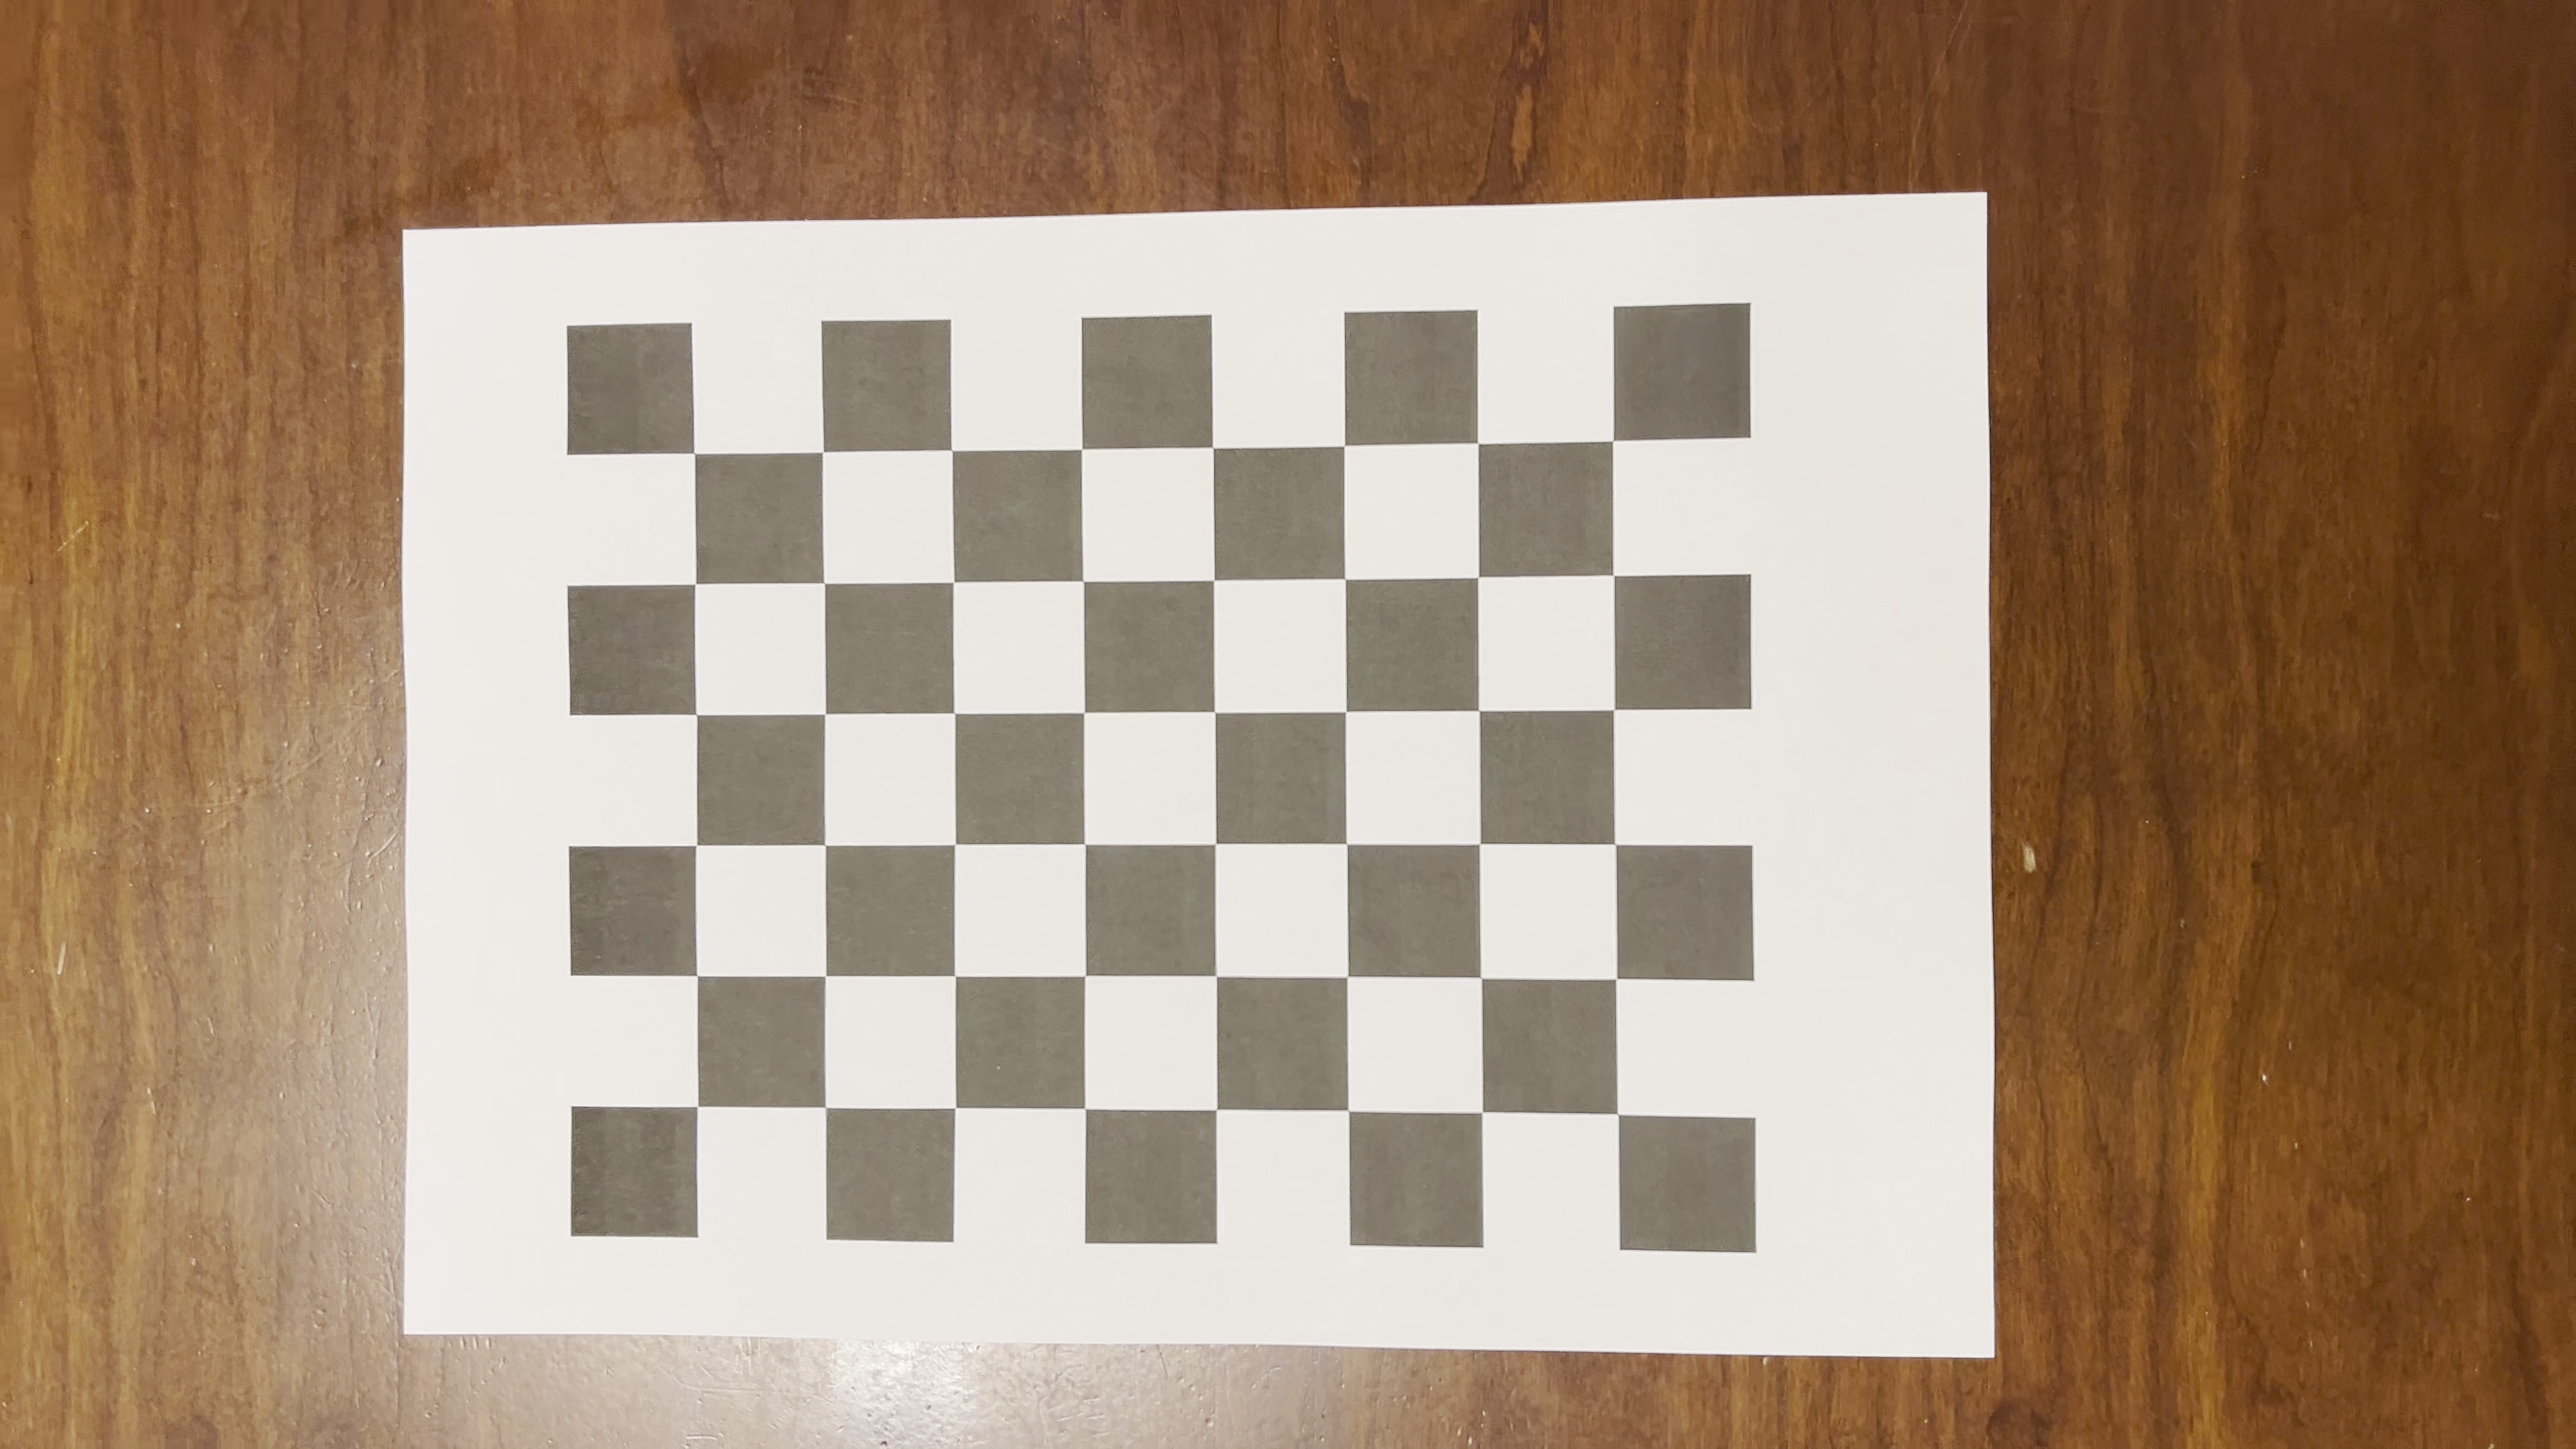
\includegraphics[width=\textwidth]{Images/checkerboard_frame_raw.png}
        \caption{Checkerboard corners detected using \texttt{cv2.findChessboardCorners}.}
        \label{fig:checkerboard-raw}
    \end{subfigure}
    \hfill
    \begin{subfigure}[b]{0.48\textwidth}
        \centering
        \includegraphics[width=\textwidth]{Images/checkerboard_frame_annotated.png}
        \caption{Detected corners annotated on frame.}
        \label{fig:checkerboard-annotated}
    \end{subfigure}

    \vspace{1em} % adjust spacing between rows

    % Bottom row: montage image
    \begin{subfigure}[b]{0.85\textwidth}
        \centering
        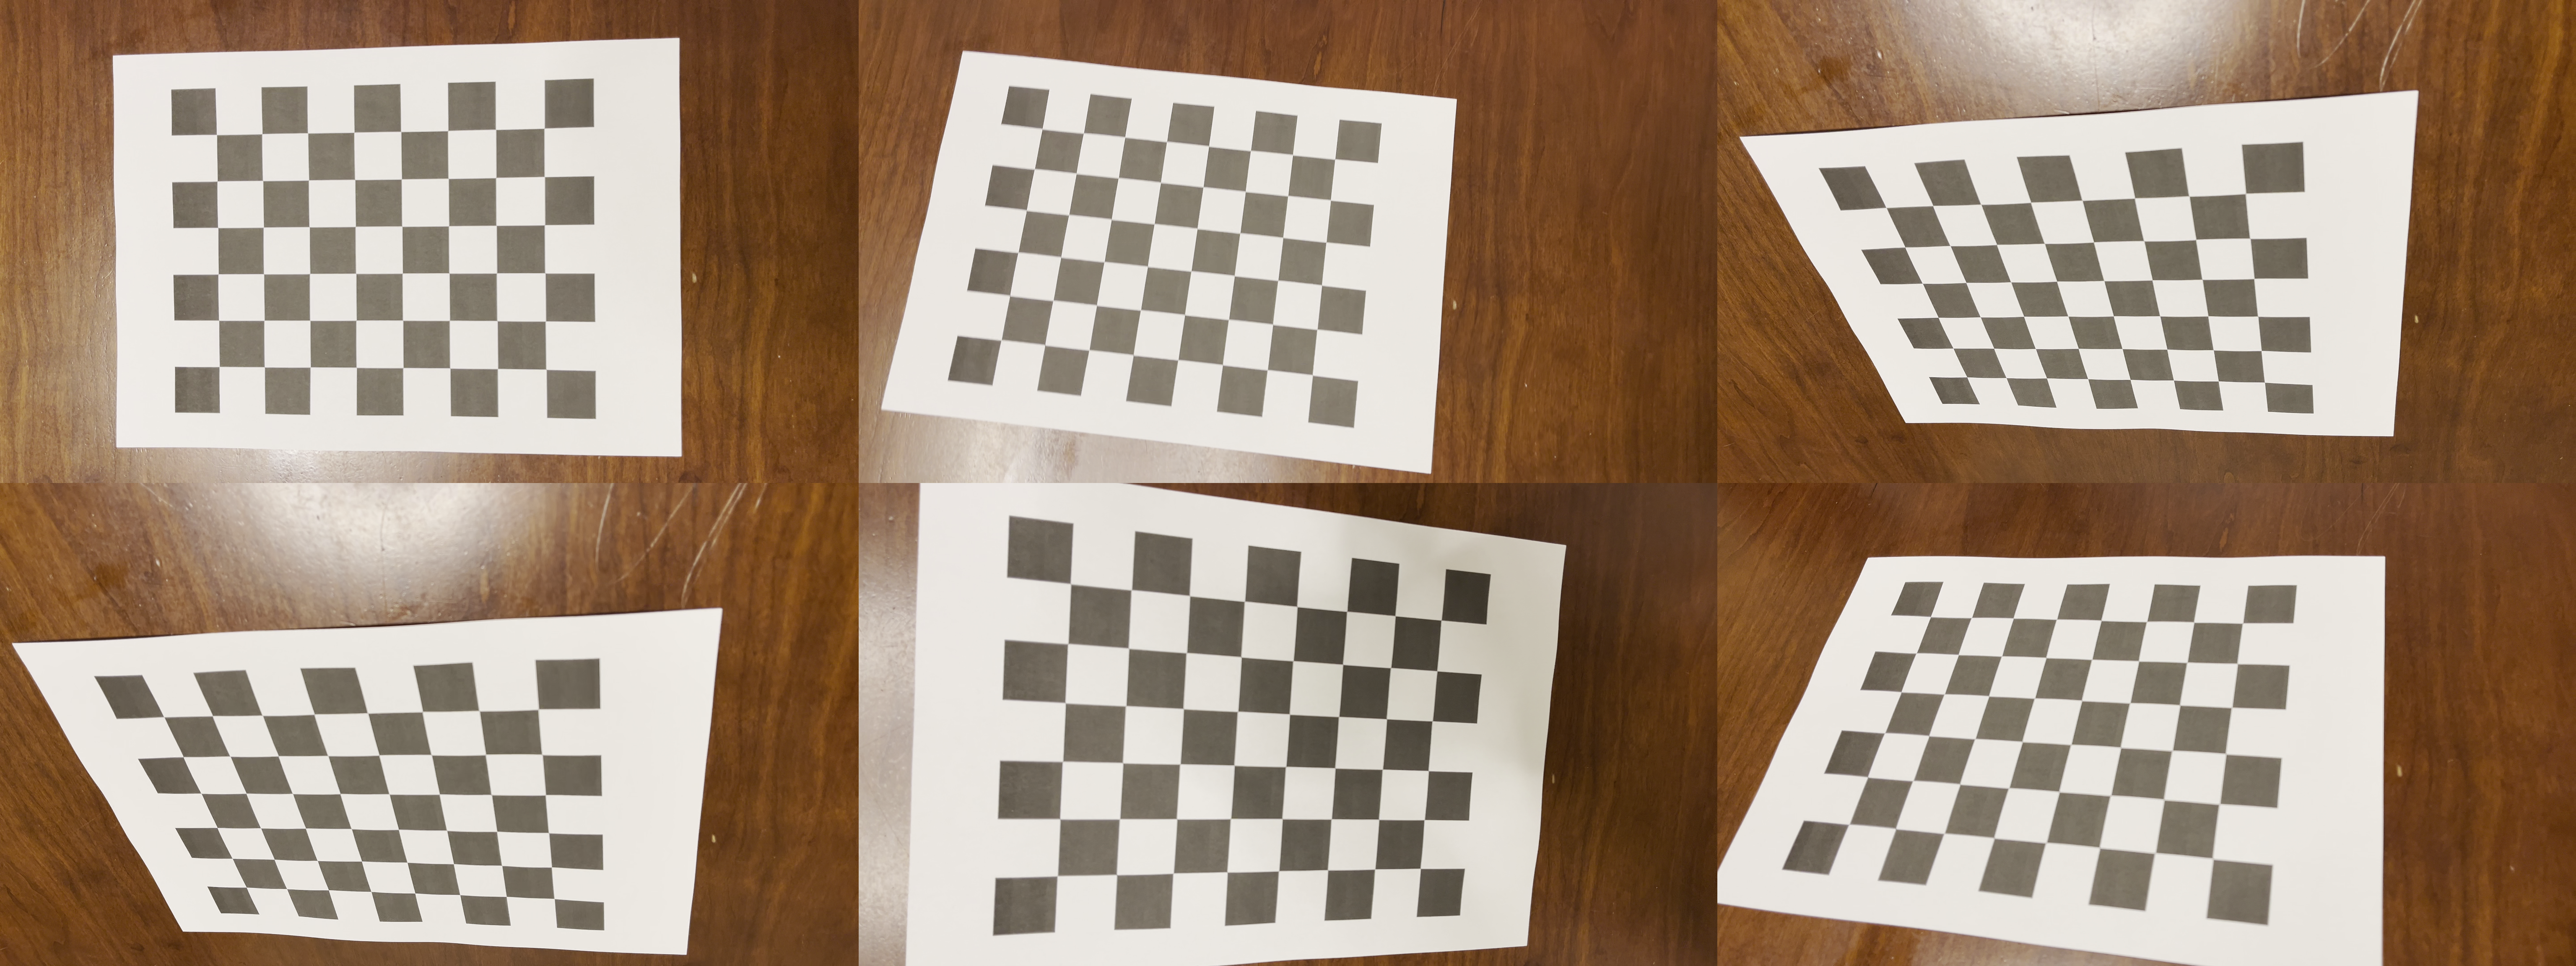
\includegraphics[width=\textwidth]{Images/checkerboard_montage.png}
        \caption{Multiple calibration views for geometric diversity.}
        \label{fig:checkerboard-diverse}
    \end{subfigure}

    \caption{Detected checkerboard corners (top) and selection of calibration frames (bottom).}
    \label{fig:checkerboard-combined}
\end{figure}

\section{Vehicle Model and Reference Dimensions}
The vehicle used as the reference model in this project is the \textbf{Škoda Fabia}. Its rear geometry was selected due to its clear symmetry, availability of technical dimensions, and suitability for feature-based pose estimation. All geometric measurements, including the positions of rear lights, license plate corners, and mirrors, were manually extracted from the official reference image and scaled to millimeters.

The following are the main physical dimensions used:

\begin{itemize}
    \item \textbf{Height of internal rear lights (A–B)}: 1000 mm
    \item \textbf{Height of external rear lights (E–F)}: 1200 mm
    \item \textbf{Height of license plate lower corners (C–D)}: 900 mm
    \item \textbf{Width of the license plate (distance C–D)}: 520 mm
    \item \textbf{Distance between internal rear lights (A–B)}: 860 mm
    \item \textbf{Distance between external rear lights (E–F)}: 1400 mm
    \item \textbf{Total vehicle width (O–F)}: 1732 mm
    \item \textbf{Wheel-to-wheel width (O–O)}: 1457 mm
    \item \textbf{Angle $\varphi$ between the vertical and the rear surface of the vehicle}: $9.46^\circ$
\end{itemize}

\begin{figure}[htbp]
    \centering
    \includegraphics[width=0.85\textwidth]{Images/cad.jpg}
    \caption{2D CAD-style schematic of the reference vehicle (Škoda Fabia), annotated with labeled feature points and known dimensions in millimeters.}
    \label{fig:car-cad-model}
\end{figure}
\chapter{Feature Extraction}
This section presents a methodology to extract geometric and photometric features of a vehicle's rear side, focusing specifically on the detection of taillights, the localization of the license plate and the localization of the side mirror from image frames. These features serve as critical landmarks for estimating the rear plane and pose of the vehicle in 3D space.

\section{Frames extraction from video}
After filming the nighttime video and calibrating the camera, we moved to extract a set of evenly spaced frames from our video file for further analysis or processing. Specifically, we opened the video, computed the total number of frames, and then selected a fixed number of frames uniformly distributed across the video timeline. We then saved the frames extracted in a folder.

Figure~\ref{fig:frames_sequence} shows four frames extracted from the original video. The symmetric taillights and the license plate are clearly visible across all frames, and serve as key features for 3D localization and orientation estimation.

\begin{figure}[h!]
    \centering
    \begin{subfigure}[b]{0.24\textwidth}
        \includegraphics[width=\textwidth]{Images/featureExtractions/frame00.jpg}
        \caption{Frame 0}
    \end{subfigure}
    \begin{subfigure}[b]{0.24\textwidth}
        \includegraphics[width=\textwidth]{Images/featureExtractions/frame04.jpg}
        \caption{Frame 4}
    \end{subfigure}
    \begin{subfigure}[b]{0.24\textwidth}
        \includegraphics[width=\textwidth]{Images/featureExtractions/frame08.jpg}
        \caption{Frame 8}
    \end{subfigure}
    \begin{subfigure}[b]{0.24\textwidth}
        \includegraphics[width=\textwidth]{Images/featureExtractions/frame12.jpg}
        \caption{Frame 12}
    \end{subfigure}

    \caption{Sequence of extracted frames used for symmetric feature tracking}
    \label{fig:frames_sequence}
\end{figure}

\section{Taillights Extraction}
The detection process begins by isolating the vehicle from the background using a convolutional neural network trained on object detection (such as YOLO). This network identifies and localizes the vehicle in each image through a bounding box. The image is then cropped to this bounding box, reducing irrelevant background content and focusing analysis on the vehicle’s rear.

Once the rear of the vehicle has been isolated, we aim at locating the red taillights. Rather than operating in RGB color space, which is sensitive to illumination changes, the image is converted to HSV (Hue, Saturation, Value). This shift is non-trivial: in HSV space, hue represents color in a more stable manner, making red easier to isolate under variable lighting conditions such as shadows, glares, or overexposure.

Two hue ranges are defined—one near 0° and another near 180°—to encompass the dual ends of the red spectrum, since taillights have a stronger red in the heart of lights and a lighter red around them. These ranges are used to create binary masks that isolate red regions. Morphological operations follow, cleaning up the masks by removing small noise and enhancing continuous regions. From here, contours are detected and filtered. The obtained mask looks as follows:

\begin{figure}[htbp]
    \centering
    \includegraphics[width=0.5\linewidth]{Images//featureExtractions/redLightsMask.png}
    \caption{Mask found for red taillights}
    \label{fig:redLightsMask}
\end{figure}

The assumption is that the two largest red regions within this refined mask correspond to the taillights. This is a reasonable consideration, especially in urban night driving scenarios where taillights are often the most prominent red features. The methodology then computes two points for each taillight: the center and the bottom outer edge. These points are not are going to serve later as structural anchors for orientation estimation and projection.

\begin{figure}[htbp]
    \centering
    \includegraphics[width=0.4\linewidth]{lightsDetection1.png}
    \caption{Example of taillights detection from a frame}
    \label{fig:lightsDetection}
\end{figure}

Using these taillight detections, the orientation of the rear plane is inferred by calculating the angle of the line joining the taillights. This angle is used to rotate the image such that the taillights lie along a horizontal axis, making subsequent feature extraction more stable and geometrically consistent.

\section{License Plate Extraction}
Following rotation, the license plate is expected to lie directly below the line connecting the taillights. A region of interest (ROI) is defined between and below the taillights to constrain the search space. Within this region, segmentation is performed to isolate the license plate, using its characteristic colour properties—primarily white for the body of the plate and blue for the side strip, as found in many European plates.

\begin{figure}[htbp]
    \centering
    \includegraphics[width=0.5\linewidth]{Images//featureExtractions/plateMask.png}
    \caption{Mask found for plate}
    \label{fig:plateMask}
\end{figure}

Contours are then extracted and ranked based on geometric properties. Among the candidates, the one with the largest area and an appropriate aspect ratio (typically between 1.5 and 5.5) is selected as the license plate. The bounding box surrounding this contour defines the spatial extent of the plate in the image.

The final output of this process is the localization of the license plate via its bounding box and the precise positions of the taillights. These elements jointly define a consistent geometric configuration on the vehicle’s rear surface and are essential for downstream tasks such as vanishing point estimation, camera resectioning, and 3D back-projection of the rear plane.

\begin{figure}[htbp]
    \centering
    \includegraphics[width=0.4\linewidth]{Images/licenceDetection1.png}
    \caption{Example of licence plate detection from a frame}
    \label{fig:licenceDetection}
\end{figure}

\section{Side Mirror Extraction}
This section outlines a procedure for detecting the side mirror of a vehicle from a single image frame. The mirror serves as a salient lateral landmark that contributes to understanding the vehicle's spatial extent and orientation in 3D space.

The process begins with isolating the vehicle from its surroundings using an object detection model based on the YOLO architecture, as in the previous section. To account for side elements like mirrors that may lie slightly outside the bounding box, the crop is expanded slightly along the horizontal axis.

Once the vehicle region is extracted, the image is preprocessed to highlight structural edges. The cropped frame is first converted to gray-scale, then smoothed using a Gaussian blur to reduce noise. This is followed by Canny edge detection, which enhances high-contrast boundaries and delineates object contours. This step ensures that only well-defined shapes—such as the mirror's outline—are retained for further analysis.

Contours are extracted from the resulting edge map and filtered to retain only those above a certain arc length threshold. This helps eliminate small and irrelevant features while preserving prominent shapes likely to correspond to vehicle components. The filtered contours are then drawn onto a blank canvas for visual inspection and geometric reasoning.

To locate the side mirror, the algorithm searches for the contour point with the most extreme horizontal (x-axis) position. This point is selected based on the assumption that the mirror protrudes outward from the main body of the vehicle and will be positioned near the outermost edge of the cropped frame.

Once identified, the position of the mirror is adjusted to match the coordinates of the original image by reapplying the offset introduced during the initial cropping. This ensures spatial consistency with other detected features.

The output is a single point representing the mirror's location in the global image frame. This point can be integrated with other detected features—such as taillights or license plates—to improve vehicle orientation estimation, determine lateral spread.

\begin{figure}[htbhp]
    \centering
    \begin{subfigure}[b]{0.32\textwidth}
        \includegraphics[width=\textwidth]{Images/featureExtractions/MirrorDetection/yolo_frame1.png}
        \caption{Cropped part}
    \end{subfigure}
    \begin{subfigure}[b]{0.32\textwidth}
        \includegraphics[width=\textwidth]{Images/featureExtractions/MirrorDetection/edges.png}
        \caption{Edges Detected}
    \end{subfigure}
    \begin{subfigure}[b]{0.32\textwidth}
        \includegraphics[width=\textwidth]{Images/featureExtractions/MirrorDetection/long_contours.png}
        \caption{Filtered Edges}
    \end{subfigure}

    \caption{Intermediate steps of side mirror detection}
    \label{fig:side-mirror-steps}
\end{figure}

\begin{figure}[htbhp]
    \centering
    \includegraphics[width=0.4\linewidth]{Images/featureExtractions/MirrorDetection/mirror_detected.png}
    \caption{Example of side mirror detection from a frame}
    \label{fig:mirrorDetection}
\end{figure}

\chapter{Methodology}
\section{Methodology Overview}
This chapter introduces the overall approach followed to estimate the space occupied by a moving vehicle using visual data acquired in low-light conditions. Based on the input video, the intrinsic calibration matrix and the extracted features obtained in the previous chapters, we developed and implemented four distinct localization methods.

Each method relies on geometric reasoning and leverages known or assumed properties of the scene, such as symmetry, planarity, or the car's motion profile. While each method aims at reconstructing the 3D position and orientation of the vehicle, they differ in the number and type of visual features used, and in their robustness to perspective limitations.

The methods presented in the following chapters are:
\begin{enumerate}
    \item \textbf{Standard localization via homography}: uses four coplanar points on the rear facade of the car (e.g., rear lights and license plate corners) to estimate pose from a single image using homography decomposition.
    
    \item \textbf{Nighttime localization from pair of images}: designed for low-light settings, this method uses symmetric rear light points tracked across two frames. It exploits temporal motion cues to estimate the pose of the vehicle on the road.
    
    \item \textbf{Localization under poor perspective using out-of-plane symmetric features}: when perspective cues are weak, this method uses symmetric features located on different planes of the car's 3D structure (e.g., lights and mirrors) to recover pose by exploiting inter-frame symmetry and vanishing geometry.

    \item \textbf{PnP-based vehicle pose estimation from key points}: this method estimates the vehicle’s 3D pose from a single image by solving the Perspective-n-Point (PnP) problem using a set of known 3D key points (e.g., rear lights, license plate corners, and side mirror) and their 2D projections. By including non-coplanar points such as the side mirror, the method improves robustness and accuracy, especially in low-perspective conditions.
\end{enumerate}

Each method is presented with its theoretical foundations, practical implementation, and a critical discussion of its applicability. Comparative results will be provided at the end to assess their relative performance and reliability in real-world conditions.

\section{Method 1: Standard localization via homography}
This method enables the estimation of a vehicle’s 3D position and orientation from a single image, under the assumption of known intrinsic camera parameters and a simplified vehicle model. The approach relies on the identification of symmetric and well-localized features—typically the rear lights and the corners of the license plate—which are assumed to lie on the vehicle's rear plane. By exploiting known real-world distances between these features, it is possible to triangulate their positions in 3D space and reconstruct a rear-facing coordinate frame aligned with the vehicle geometry. The final output is a 3D bounding box that approximates the vehicle's occupied space. While this method requires only a single frame, its performance is highly sensitive to feature localization accuracy and the presence of sufficient perspective distortion in the image.

\subsection{Theoretical Foundations}
The mathematical framework underlying the method is founded on three pillars of projective geometry and photogrammetry.

\subsubsection{Pinhole Camera Model and Back-Projection}
A standard pinhole camera model is adopted, where the transformation from a 3D point in the camera space, $\mathbf{P} = [X, Y, Z]^T$, to an image point in homogeneous coordinates, $\tilde{\mathbf{x}} = [u, v, w]^T$, is described by the intrinsic matrix $K \in \mathbb{R}^{3 \times 3}$:
\[
\lambda \tilde{\mathbf{x}} = K \mathbf{P}
\]
where $\lambda$ represents the scene depth. The inverse operation, or \textbf{back-projection}, is essential for 3D reconstruction. Given an image point $\mathbf{x}_{pix}$, its homogeneous coordinates $\tilde{\mathbf{x}}$ are mapped to a 3D directional ray $\mathbf{d}$ in the camera space, according to the relation:
\[
\mathbf{d} = K^{-1} \tilde{\mathbf{x}}
\]
This vector $\mathbf{d}$ defines the line on which the 3D point $\mathbf{P}$ lies, but not its exact position along it.

\subsubsection{Triangulation with Geometric Constraints}
To resolve the depth ambiguity, a metric constraint is introduced, namely a known real-world distance such as the license plate width, $w_{plate}$. Given two image points $p_0$ and $p_1$ and their corresponding normalized 3D rays $\mathbf{d}_0$ and $\mathbf{d}_1$, they form a triangle with the camera center. The angle $\theta$ between the two rays can be calculated via the dot product:
\[
\theta = \arccos(\mathbf{d}_0 \cdot \mathbf{d}_1)
\]
Assuming that the two 3D points $\mathbf{P}_0$ and $\mathbf{P}_1$ are at approximately the same depth from the camera, the triangle formed by $\mathbf{P}_0$, $\mathbf{P}_1$, and the camera center can be approximated as isosceles. The average depth $d$ can then be estimated geometrically:
\[
d_{approx} = \frac{w_{plate}}{2 \sin(\theta / 2)}
\]
This estimate is subsequently refined to ensure that the Euclidean distance between the reconstructed 3D points, $\mathbf{P}_0 = d_0 \mathbf{d}_0$ and $\mathbf{P}_1 = d_1 \mathbf{d}_1$, exactly satisfies the constraint $\|\mathbf{P}_1 - \mathbf{P}_0\| = w_{plate}$.

\subsubsection{Vanishing Point Geometry}
The vehicle's orientation is recovered by exploiting the properties of vanishing points. In projective geometry, parallel lines in 3D space appear to converge to a single point on the image plane, known as the vanishing point. By identifying two or more lines on the image known to be parallel in reality (e.g., the top and bottom edges of the license plate), their intersection point $\mathbf{v_p}$ can be computed. The back-projection of $\mathbf{v_p}$ yields a 3D vector $\mathbf{v}_{dir}$ that indicates the direction of these parallel lines in the camera space, corresponding to the vehicle's longitudinal axis.
\[
\mathbf{v_p} = l_1 \times l_2 \quad \implies \quad \mathbf{v}_{dir} = K^{-1} \mathbf{v_p}
\]

\subsubsection{Algorithmic Pipeline}
The implementation of the method follows a defined sequence of operations.

\begin{enumerate}
    \item \textbf{Preprocessing and Feature Extraction}: The image is corrected for optical distortions using known calibration parameters ($K$, \texttt{dist}). Subsequently, four coplanar keypoints are extracted: two corners of the license plate (\texttt{TL}, \texttt{TR}) and the two taillights (\texttt{L2}, \texttt{R2}). The coordinates of these points are also undistorted.

    \item \textbf{3D Point Reconstruction}: The \texttt{triangulate\_plate\_points} function implements the constrained triangulation described above to compute the 3D coordinates, $\mathbf{P}_0$ and $\mathbf{P}_1$, of the license plate corners.

    \item \textbf{Vanishing Point Estimation}: The function \texttt{compute\_vanishing\_direction} calculates the intersection of two lines in the image: the first connects the license plate corners (points \texttt{TL} and \texttt{TR}), and the second connects the taillights (points \texttt{L2} and \texttt{R2}). These lines, assumed to be parallel in the real world, intersect in the image due to perspective projection. Their intersection defines a vanishing point $\mathbf{v_p}$ in the image plane, which is then back-projected into a 3D direction vector $\mathbf{v}_{dir} = K^{-1} \mathbf{v_p}$ that approximates the vehicle's forward direction in the camera coordinate frame.

    \item \textbf{Vehicle Coordinate Frame Construction}: The \texttt{build\_vehicle\_frame} function establishes a local coordinate system attached to the vehicle.
    
    \begin{itemize}
        \item \textbf{X-axis}: Defined as the unit vector connecting the two 3D license plate points, $\mathbf{x}_{axis} = \text{normalize}(\mathbf{P}_1 - \mathbf{P}_0)$.
        \item \textbf{Y-axis}: Calculated from the vanishing point direction $\mathbf{v}_{dir}$, made orthogonal to $\mathbf{x}_{axis}$ through a Gram-Schmidt orthogonalization process.
        \item \textbf{Z-axis}: Obtained via the cross product $\mathbf{z}_{axis} = \text{cross}(\mathbf{x}_{axis}, \mathbf{y}_{axis})$ to form a right-handed coordinate system.
        \item \textbf{Origin}: Placed at the center of the license plate segment, then translated along the local Z-axis.
        \item \textbf{Rotation Matrix}: The vehicle's rotation matrix $R$ relative to the camera is constructed by stacking the three axes as columns: $R = [\mathbf{x}_{axis} | \mathbf{y}_{axis} | \mathbf{z}_{axis}]$.
    \end{itemize}

    \item \textbf{3D Bounding Box Generation}: The 8 vertices of the cuboid are defined in the vehicle's local coordinates, based on its known dimensions. Each local vertex $\mathbf{p}_{local}$ is then transformed into the camera's coordinate system using the estimated pose (rotation $R$ and translation origin): $\mathbf{p}_{camera} = R \mathbf{p}_{local} + \text{origin}$.
\end{enumerate}

\subsection{Results and Discussion}
The outcome of this method is shown in Figure~\ref{fig:method1_result}. While the reconstructed bounding box follows the expected geometric structure, the projected result shows visible misalignment with the actual vehicle in the image. This discrepancy is primarily attributed to insufficient perspective in the observed view, which limits the accuracy of depth estimation during triangulation. In particular, nearly frontal or rear views result in collinear or weakly separated viewing rays, making depth inference unstable. Furthermore, small localization errors in selecting the symmetric features—especially the taillights points can lead to amplified inaccuracies in the 3D reconstruction. These limitations motivated the development of more robust techniques described in the subsequent sections.

\begin{figure}[htbp]
    \centering
    \includegraphics[width=0.30\textwidth]{Images/method1/bbox1.jpg}
    \caption{Projection of the estimated 3D bounding box using the single-frame localization method. Weak perspective and minor feature localization errors affect the accuracy.}
    \label{fig:method1_result}
\end{figure}


\section{Method 2: Nighttime localization from pair of images}
\subsection{Introduction}
This method aims to localize a vehicle at night by using a pair of images taken at different time instances (non consecutive). Unlike standard object detection methods, this approach leverages geometric reasoning and camera calibration to estimate the 3D position and orientation of the vehicle using only the taillights visible in nighttime conditions. The technique relies on identifying two pairs of corresponding symmetric points (in our case the taillights) on the rear of a moving vehicle in two non consecutive frames and applies principles from projective geometry and perspective analysis to infer spatial information.

\subsection{Methodology}

Knowing that the camera calibration matrix was previously computed, and having previously found the rear lights reference points, we define the image points as follows:
\[
\text{Left taillight: } L_1, \quad \text{Right taillight: } R_1 \quad \text{(frame 1)}
\]
\[
\text{Left taillight: } L_2, \quad \text{Right taillight: } R_2 \quad \text{(frame 2)}
\]

We then consider these image points in homogeneous coordinates:
\[
\tilde{L}_1 = \begin{bmatrix} x_{L_1} \\ y_{L_1} \\ 1 \end{bmatrix}, \quad \tilde{R}_1 = \begin{bmatrix} x_{R_1} \\ y_{R_1} \\ 1 \end{bmatrix}, \quad \tilde{L}_2 = \begin{bmatrix} x_{L_2} \\ y_{L_2} \\ 1 \end{bmatrix}, \quad \tilde{R}_2 = \begin{bmatrix} x_{R_2} \\ y_{R_2} \\ 1 \end{bmatrix}
\]

\subsubsection{Vanishing points and vehicle motion}
Two vanishing points needed for this method, are computed as:
\begin{itemize}
    \item \( V_x \): from the intersection of the taillight segments in each of the two frames:
    \[
    \ell_1 = \tilde{L}_1 \times \tilde{R}_1, \quad \ell_2 = \tilde{L}_2 \times \tilde{R}_2
    \]
    \[ \quad V_x = \ell_1 \times \ell_2
    \]
    \item \( V_y \): from the intersection of two left rear lights, and two right rear lights of the two frames:
    \[
    \ell_L = \tilde{L}_1 \times \tilde{L}_2, \quad \ell_R = \tilde{R}_1 \times \tilde{R}_2 \]
    \[\quad V_y = \ell_L \times \ell_R
    \]
\end{itemize}

These vanishing points are back-projected into the camera coordinate system using the inverse of the calibration matrix \( K \).

\[
\vec{d}_x = K^{-1} V_x, \quad \vec{d}_y = K^{-1} V_y
\]

This operation yields direction vectors, called \textit{back-projected rays}, which represent the 3D directions in space corresponding to the vanishing points observed in the image. Each ray originates from the camera center and points along the direction in which a set of 3D parallel lines project to the same vanishing point in the image. These rays are then normalized to unit vectors for the next geometric computation.

\[
\vec{d}_x = \frac{\vec{d}_x}{\|\vec{d}_x\|}, \quad \vec{d}_y = \frac{\vec{d}_y}{\|\vec{d}_y\|}
\]

The vehicle motion is assumed to be straight (no steering) if:
\[
\vec{d}_x \cdot \vec{d}_y \approx 0
\]

which we checked in our code confirming our assumption.

\subsubsection*{3D Reconstruction of rear plane and depth estimation}

% da rivedere 

To estimate the 3D position and orientation of the vehicle's rear plane, we exploit the geometric structure observed in a pair of images and the known camera calibration matrix \( K \in \mathbb{R}^{3 \times 3} \). We consider 3D world points \( \mathbf{X} \in \mathbb{R}^3 \) project onto 2D image points \( \mathbf{x} \in \mathbb{P}^2 \) according to the mapping:
\[
\tilde{\mathbf{x}} \sim K [R \, | \, t] \mathbf{X}
\]
In our case, since we are working with fixed world geometry (i.e., the rear of the car) and trying to estimate depth and orientation, we simplify the analysis to the single-camera frame and image geometry.

\paragraph{Vanishing line of the rear plane}
The vehicle’s rear is a planar surface, and it is observed in perspective, which introduces converging lines. In projective geometry, the intersection points of pairs of corresponding lines on this plane define \textbf{vanishing points} directions of parallel lines in 3D space. We identify two vanishing points:

\begin{itemize}
\item \( V_x \): from horizontal taillight edges (width-wise direction),
\item \( V_y \): from vertical motion of taillights between frames (depth-wise motion).
\end{itemize}

The \textbf{vanishing line} \( \ell \) of the rear plane is obtained as the cross product of the two vanishing points in homogeneous image coordinates:

\[
\ell = V_x \times V_y
\]

This line represents the intersection of the rear plane with the image plane, meaning it contains all the vanishing points of lines lying on the rear surface.

\paragraph{Computing the normal plane}
In projective geometry and camera imaging, every line \( \ell \) in the 2D image corresponds to a 3D plane in space that passes through the camera’s optical center and contains all the projecting rays onto that line. This is because the camera center is a fixed point in 3D space, and all points along the image line are projections of 3D points lying on some plane intersecting the camera center.

The vanishing line \( \ell \), defined as the cross product of two vanishing points \( V_x \) and \( V_y \):
\[
\ell = V_x \times V_y
\]
represents the image of the rear plane of the vehicle. Intuitively, this line corresponds to the horizon line of that plane in the image, containing all vanishing points of directions lying on the rear surface.

To determine the orientation of this plane in 3D, we back-project the image line \( \ell \) into the camera coordinate system using the transpose of the camera intrinsic matrix \( K \):
\[
\vec{n} = K^\top \ell
\]
This operation produces a vector \( \vec{n} \) that is \textbf{normal} (perpendicular) to the corresponding 3D plane in the camera coordinate frame.

\begin{figure}
    \centering
    \includegraphics[width=0.75\linewidth]{Images/vanishing_line_method2.png}
    \caption{Lights segments and resulting vanishing line.}
    \label{fig:vanLine1}
\end{figure}

This result can be understood by considering the duality between points and lines in projective geometry, combined with the role of the intrinsic matrix \( K \):

\begin{itemize}
    \item The intrinsic matrix \( K \) maps a 3D direction vector \( \mathbf{d} \) expressed in the camera coordinate system to its corresponding point \( \tilde{\mathbf{p}} \) in the normalized image plane through the relation:
    \[
    \tilde{\mathbf{p}} = K \mathbf{d}
    \]
    Here, \( \tilde{\mathbf{p}} \) is a homogeneous 2D image point (or vanishing point) representing the projection of the 3D direction.

    \item Lines in the image, such as \( \ell \), are represented as vectors orthogonal to points (in the dual projective space). When we want to find the 3D plane corresponding to an image line, we need to "lift" this line back into 3D space.

    \item The transpose \( K^\top \) operates on image lines \( \ell \) to map them back into 3D vectors normal to the planes whose images they represent. More formally, since \( \ell \) satisfies \( \ell^\top \tilde{\mathbf{p}} = 0 \) for all points \( \tilde{\mathbf{p}} \) on that line, applying \( K^\top \) to \( \ell \) produces a vector \( \vec{n} \) such that:
    \[
    \vec{n}^\top \mathbf{d} = 0
    \]
    for all directions \( \mathbf{d} \) whose image points lie on \( \ell \).

    Thus, \( \vec{n} = K^\top \ell \) defines the normal vector to the 3D plane associated with the image line \( \ell \).
\end{itemize}


Since \( \vec{n} \) is defined up to scale, it is normalized to obtain a unit normal vector:
\[
\vec{n} = \frac{\vec{n}}{\|\vec{n}\|}
\]

The normalized vector \( \vec{n} \) thus precisely encodes the orientation of the vehicle’s rear plane relative to the camera frame. It points orthogonally outward from the rear surface, enabling further computations such as projecting points onto the plane or estimating distances from the camera.


\paragraph{Back-projected rays to the taillights}

Next, we compute the direction vectors from the camera center to the left and right taillights in the image. These are known as \textbf{back-projected rays}, obtained by applying the inverse of the calibration matrix to the image points:

\[
\vec{r}_{L_1} = \frac{K^{-1} \tilde{L}_1}{\|K^{-1} \tilde{L}_1\|}, \quad 
\vec{r}_{R_1} = \frac{K^{-1} \tilde{R}_1}{\|K^{-1} \tilde{R}_1\|}
\]

Each ray represents the direction in 3D along which a taillight lies, assuming the scene is rigid and the taillight is a fixed point in the world.

\paragraph{Angle between rays and depth estimation}

Given these rays, the angular separation between them in 3D space encodes information about the apparent size of the taillight segment. The angle \( \theta \) between the rays is computed via the dot product:

\[
\cos(\theta) = \vec{r}_{L_1} \cdot \vec{r}_{R_1}, \quad 
\theta = \arccos(\cos(\theta))
\]

This angle tells us how "wide" the taillight separation appears from the camera’s point of view. Given the \textbf{real-world width} \( w \) between the taillights (e.g., from CAD data), we can apply a simple geometric principle to estimate the depth \( d \) of the car's rear from the camera:

\[
d = \frac{w}{2 \sin(\theta / 2)}
\]

This formula arises from the \textbf{law of sines} in triangle geometry. The rays \( \vec{r}_{L_1} \) and \( \vec{r}_{R_1} \) define a triangle with a known base \( w \) and angle \( \theta \) at the vertex (camera center). The depth \( d \) corresponds to the distance from the camera to the base of the triangle, projected along the median ray.

\subsubsection{3D reconstruction and bounding box}

3D coordinates of the taillights:
\[
\vec{P}_{L_1} = d \cdot \vec{r}_{L_1}, \quad \vec{P}_{R_1} = d \cdot \vec{r}_{R_1}
\]

The midpoint between taillights is:
\[
\vec{C}_{\text{rear}} = \frac{\vec{P}_{L_1} + \vec{P}_{R_1}}{2}
\]

The rear ground contact point is computed by shifting vertically:
\[
\vec{C}_{\text{ground}} = \vec{C}_{\text{rear}} + h \cdot \vec{n}
\]
where \( h \) is the taillight height from the ground.

The local coordinate frame of the vehicle is defined as:
\[
\text{Forward: } \vec{f} = \vec{d}_y \] \[\text{right: } \vec{r} = \frac{\vec{r}_{R_1} - \vec{r}_{L_1}}{\|\vec{r}_{R_1} - \vec{r}_{L_1}\|} \]

\[\text{up: } \vec{u} = \vec{n}
\]

Using the vehicle’s CAD dimensions (length \( l \), width \( w \), height \( h \)), we are able to construct the 8 corners of the 3D bounding box.

\subsubsection{Projection and visualization}

Each 3D corner \( \vec{P}_i \) is projected into 2D image space as:
\[
\tilde{p}_i = K \vec{P}_i, \quad p_i = \left( \frac{\tilde{p}_i[0]}{\tilde{p}_i[2]}, \frac{\tilde{p}_i[1]}{\tilde{p}_i[2]} \right)
\]

Figure~\ref{fig:method2_result} shows the final result of the pose estimation using only rear taillight cues under nighttime conditions.

\begin{figure}[H]
    \centering
    \includegraphics[width=0.75\linewidth]{bb_method2.png}
    \caption{Bounding box resulting from method 2}
    \label{fig:method2_result}
\end{figure}

\section{Method 3: Poor perspective localization using out-of-plane features}
\subsection{Introduction}
The theoretical foundation of Method 3 addresses the fundamental limitation of standard homography-based localization when perspective effects are insufficient. As demonstrated in the professor's slides, the standard homography-based method can fail with poor perspective, particularly when vanishing points are close to infinity, necessitating an iterative approach that can handle such degenerate cases.

\subsection{Theoretical framework}
\subsubsection{Geometric foundation and the poor perspective problem}
The core geometric insight behind this method is the reduction of the full 3D-to-2D projection problem to a simplified 2D-to-1D projection problem, involving a single unknown parameter: the rotation angle $\theta$ between the camera's $x$-axis and the direction of the vehicle's lateral axis (i.e., the direction of segment $AB$ or $CD$). Following the professor's methodology, rather than using the actual 3D points $E$, $A$, $B$, and $F$, the method considers vertically translated versions of these points whose $z$-coordinates match the $z$-coordinate of the camera center $O$, thus projecting them onto a horizontal plane through $O$.

\begin{figure}[h]
    \centering
    \includegraphics[width=0.6\textwidth]{Images/method3/schema.jpg}
    \caption{Top-view schematic showing camera center $O$, vehicle direction, and rotation angle $\theta$}
    \label{fig:theta_top_view}
\end{figure}

This transformation simplifies the projection model: since all model points now lie on a horizontal plane through the camera center, the problem reduces to estimating a 2D-to-1D projection governed by the single angle $\theta$, which can be recovered through geometric constraints.

\subsubsection{Iterative pose estimation framework}
The method employs an iterative refinement loop that alternates between enforcing geometric constraints and updating pose parameters. While individual geometric cues may be unreliable under poor perspective, their integration into a global iterative system yields a robust and solvable estimation framework.

\paragraph{Triangulation with known distances}
Given two image points with a known 3D separation, triangulation is used to recover their 3D positions. For points $A$ and $B$ with known distance $\texttt{AB\_distance}$ and estimated direction $\mathbf{u}_{AB}$, we solve:

\begin{equation}
    t \cdot \mathbf{r}_A - s \cdot \mathbf{r}_B = \texttt{AB\_distance} \cdot \mathbf{u}_{AB}
\end{equation}

where $\mathbf{r}_A$ and $\mathbf{r}_B$ are the normalized camera rays from back-projection, and $t$, $s$ are depth scalars.

\paragraph{Back-plane normal computation}
The orientation of the vehicle’s back plane is obtained from triangulated 3D points. For example, using points $A$, $B$, $C$, and $D$:

\begin{equation}
    \mathbf{n}_{\text{back}} = \texttt{normalize} \left( ( \mathbf{B}_{3d} - \mathbf{A}_{3d} ) \times ( \mathbf{D}_{3d} - \mathbf{C}_{3d} ) \right)
\end{equation}

\paragraph{Camera vertical direction}
The vertical direction of the camera is computed by rotating the back-plane normal $\mathbf{n}_{\text{back}}$ around the vehicle’s lateral axis $\mathbf{u}_{\text{dir}}$ by the known inclination angle $\phi$:

\begin{equation}
    \mathbf{v}_{\text{cam}} = \cos(\phi) \cdot \mathbf{n}_{\text{back}} + 
    \sin(\phi) \cdot ( \mathbf{u}_{\text{dir}} \times \mathbf{n}_{\text{back}} ) + 
    (1 - \cos(\phi)) \cdot \langle \mathbf{u}_{\text{dir}}, \mathbf{n}_{\text{back}} \rangle \cdot \mathbf{u}_{\text{dir}}
\end{equation}

\subsubsection{Horizon Line Projection and $\theta$ Computation}
A key step in the estimation pipeline involves projecting selected image points onto the horizon line to extract the yaw angle $\theta$.

\paragraph{Vertical Vanishing Point}
The vertical vanishing point $\mathbf{V}_z$ is computed from the camera's vertical direction:

\begin{equation}
    \mathbf{V}_z = \mathbf{K} \cdot \mathbf{v}_{\text{cam}}
\end{equation}

\paragraph{Horizontal Vanishing Line}
The horizon line $l_\infty$ is derived from the same vertical direction:

\begin{equation}
    l_\infty = \mathbf{K}^{-T} \cdot \mathbf{v}_{\text{cam}}
\end{equation}

\paragraph{Horizon Projection}
Each image point is projected onto the horizon by computing the intersection of the vertical line through $\mathbf{V}_z$ with $l_\infty$:

\begin{equation}
    \texttt{point\_on\_horizon} = (\mathbf{V}_z \times \mathbf{p}) \times l_\infty
\end{equation}

\paragraph{Yaw Angle Computation}
Once points $A''$ and $B''$ are projected on the horizon, the angle $\theta$ is extracted as:

\begin{equation}
    \theta = \arctan2( B''_y - A''_y, B''_x - A''_x )
\end{equation}

\subsubsection{Convergence and Stability}
The iterative algorithm converges by repeatedly satisfying the above constraints while adjusting the estimated angle and geometric parameters.

\subsection{Methodology}
\subsubsection{Initial Pose Estimation from Rear Plane Features}
The process begins with a coarse pose estimation using four coplanar points on the rear facade of the car—rear lights (A, B) and license plate corners (C, D). This estimate is based on vanishing point analysis: the lateral vanishing point $V_x$ is obtained from the intersection of the lines AB and CD and then back-projected using the camera matrix $K$ to obtain the lateral direction in 3D. Although this estimate is often inaccurate under poor perspective, it establishes a geometrically consistent initialization, including the back-plane normal and a first approximation of the camera’s vertical direction.

\subsubsection{Triangulation with Known Physical Constraints}
Once symmetric 2D points and their real-world distances are known from the vehicle CAD model, triangulation is used to reconstruct their 3D coordinates. The method back-projects the points to normalized rays and solves for depths that satisfy both the projection geometry and the known distance between points:

\begin{equation}
    t \cdot \mathbf{r}_A - s \cdot \mathbf{r}_B = \texttt{AB\_distance} \cdot \mathbf{u}_{AB}
\end{equation}

This constrained triangulation ensures physical plausibility and geometric consistency with the vehicle model even in the presence of poor perspective or noisy detections.

\subsubsection{Horizon Line Projection and Yaw Angle Computation}
The yaw angle $\theta$ is refined by projecting selected image points onto the horizon line. The vertical vanishing point $V_z$ is computed from the rotated back-plane normal using Rodrigues' formula. The horizontal vanishing line $l_\infty$ is then computed from $V_z$ and the calibration matrix $K$.

Each image point is projected onto $l_\infty$ by intersecting the vertical line through $V_z$ with the horizon line:

\begin{equation}
    \texttt{point}_{\text{horizon}} = (\mathbf{V}_z \times \mathbf{p}) \times l_\infty
\end{equation}

The yaw angle $\theta$ is then computed between projected points (e.g., $A''$, $B''$):

\begin{equation}
    \theta = \arctan2( B''_y - A''_y, B''_x - A''_x )
\end{equation}

When multiple symmetric pairs are available, a circular mean is used to robustly estimate the average yaw angle.

\subsubsection{Iterative Refinement Framework}
The core refinement loop performs the following updates at each iteration:

\begin{itemize}
    \item Update vehicle lateral direction (direction along $X$ axis) using the current $\theta$
    \item Perform triangulation using updated rays and known distances
    \item Refine the back-plane normal via cross product or SVD
    \item Rotate the back-plane normal to compute the new vertical direction
    \item Recompute vanishing geometry ($V_z$, $l_\infty$)
    \item Project symmetric points onto $l_\infty$ and update $\theta$
\end{itemize}

The updated yaw estimates are averaged using circular statistics. The loop continues until convergence criteria are met—either a small enough change in $\theta$, consistent geometry, or a max iteration count.

\subsection{Results and Evaluation}
The proposed method was evaluated on a test frame under poor perspective conditions, using the rear lights, license plate corners, and external rear lights (E–F) as symmetric features for pose estimation.

\subsubsection{Iterative Yaw Angle Convergence}
The method started from an initial yaw angle estimate of $\theta_{\text{init}} = 9.46^\circ$. Through the iterative refinement loop, the angle was progressively updated based on vanishing geometry and horizon line projections. The convergence log is as follows:

\begin{itemize}
    \item Iteration 1: $\theta = 6.27^\circ$, $\Delta\theta = -2.34^\circ$
    \item Iteration 2: $\theta = 5.89^\circ$, $\Delta\theta = -1.88^\circ$
    \item Iteration 3: $\theta = 5.58^\circ$, $\Delta\theta = -1.55^\circ$
    \item Iteration 4: $\theta = 4.37^\circ$, $\Delta\theta = -1.28^\circ$
    \item Iteration 5: $\theta = 4.17^\circ$, $\Delta\theta = -0.21^\circ$
    \item Iteration 6: $\theta = 4.14^\circ$, $\Delta\theta = -0.04^\circ$
\end{itemize}

The process converged after 7 iterations, yielding a final yaw estimate of $\theta_{\text{final}} = \mathbf{4.14^\circ}$. This demonstrates the effectiveness of the proposed method in refining vehicle orientation even under weak perspective cues.

\subsubsection{Geometric Consistency of Triangulated Features}

The method achieves high consistency between the triangulated 3D distances and the real-world measurements from the CAD model:

\begin{center}
    \begin{tabular}{lcc}
        \toprule
        \textbf{Feature Pair} & \textbf{Computed Distance (m)} & \textbf{Expected Distance (m)} \\
        \midrule
        A--B (rear lights, internal) & 0.860 & 0.86 \\
        C--D (license plate corners) & 0.520 & 0.52 \\
        E--F (rear lights, external) & 1.400 & 1.40 \\
        \bottomrule
    \end{tabular}
\end{center}

This confirms that the triangulation module, guided by the estimated yaw and direction vector, remains geometrically reliable.

\subsubsection{Final Projection Result}
Figure~\ref{fig:method3_result} shows the final result of the pose estimation: a 3D bounding box is projected onto the image using the computed pose and the simplified car model. The orientation aligns visually with the vehicle's position, confirming the correctness of the yaw and translation estimation.

\begin{figure}[h]
    \centering
    \includegraphics[width=0.35\textwidth]{Images/method3/final_bounding_box_method3.jpg}
    \caption{Final pose estimation result using Method 3. The bounding box aligns with the car's geometry, demonstrating successful localization under poor perspective.}
    \label{fig:method3_result}
\end{figure}

\section{Method 4: PnP-based vehicle pose estimation from key points}
\subsection{Introduction}
This method leverages the Perspective-n-Point (PnP) problem to estimate the 3D pose of a vehicle from a single image frame. Unlike homography-based approaches, PnP allows for accurate reconstruction even when using out-of-plane points, such as the side mirror. The method is implemented in two main variants: one using 4 coplanar points (rear lights and license plate), and another using 5 points, including the mirror, to assess the impact of additional 3D depth on localization accuracy.

\subsection{Theoretical framework}
\subsubsection{The perspective-n-point problem}
The PnP problem involves estimating the position and orientation (pose) of a camera relative to a known 3D object, given:
\begin{itemize}
    \item A set of $n \geq 4$ known 3D points in the object coordinate system,
    \item Their corresponding 2D projections in the image plane,
    \item The camera's intrinsic matrix $K$.

\end{itemize}

Mathematically, the PnP problem seeks to find the rotation matrix $\mathbf{R} \in SO(3)$ and translation vector $\mathbf{t} \in \mathbb{R}^3$ that satisfy the camera projection equation:
\begin{equation}
    s \cdot \mathbf{p}_i = \mathbf{K} \cdot [\mathbf{R}|\mathbf{t}] \cdot \mathbf{P}_i
\end{equation}
where $\mathbf{p}_i$ represents the 2D image coordinates, $\mathbf{P}_i$ the corresponding 3D world coordinates, $\mathbf{K}$ the camera intrinsic matrix, and $s$ a scale factor. The rotation matrix $\mathbf{R}$ belongs to the \textit{Special Orthogonal Group} $SO(3)$, which denotes the set of all $3 \times 3$ orthogonal matrices with determinant equal to 1. This constraint ensures that $\mathbf{R}$ represents a proper rotation in 3D space, preserving lengths and angles without reflection. 

\subsubsection{PnP vs homography}
The main distinction between PnP and homography methods (\texttt{findHomography}) lies in their assumptions:
\begin{itemize}
    \item Homography assumes that all 3D points lie on the same plane (planar geometry).
    \item PnP makes no such assumption and performs well even with non-coplanar configurations. It is thus more robust in low-perspective conditions or when using points with different depths.
\end{itemize}

\subsubsection{PnP algorithm variants}
Modern PnP solvers employ different strategies for pose estimation. \textbf{Iterative PnP} methods require an initial pose estimate and refine it through non-linear optimization, typically providing higher accuracy when a reasonable initialization is available. \textbf{EPnP (Efficient PnP)} solvers, implemented through the \texttt{SOLVEPNP\_EPNP} method, compute the pose using a non-iterative approach based on expressing 3D points as weighted sums of four virtual control points. This method offers computational efficiency and numerical stability without requiring initial pose estimates, making it particularly suitable for real-time applications. \textbf{PnPRANSAC} combines pose estimation with robust outlier detection using random sample consensus, making it suitable for noisy feature correspondences where some point matches may be incorrect.

\subsection{Methodology}
\subsubsection{Four-point PnP approach: license plate and taillights}
The first methodology employs a four-point correspondence system utilizing the vehicle's license plate and taillights positions. This approach leverages the geometric regularity and predictable spatial relationships of these vehicle features to establish reliable 3D-to-2D point correspondences.
\paragraph{Feature point selection and 3D model definition}
The 3D vehicle model is defined using four key reference points:
\begin{itemize}
    \item \textbf{License plate corners}: two points representing the lower corners of the rear license plate.
    \item \textbf{Taillights points}: two points representing the rear taillights.
\end{itemize}
\paragraph{PnP solver implementation and comparison}
Two distinct PnP solving strategies were implemented and evaluated:
\begin{itemize}
    \item \textbf{Iterative PnP with initial pose estimation}: This approach first computes a rough pose estimate using analytical methods, then refines this estimate through iterative optimization. The initial pose is derived from the license plate plane geometry, providing a stable starting point for convergence.
    \item \textbf{Direct PnP solution}: This method computes the pose directly from the four-point correspondences without requiring initialization. The solver employs robust estimation techniques to handle potential noise and outliers in the feature detection process.
\end{itemize}

Experimental evaluation revealed that both approaches converge to nearly identical solutions when applied to the same feature correspondences.

\subsubsection{Five-point PnP approach: enhanced model with mirror integration}
To improve pose estimation accuracy and provide additional geometric constraints, we extended the methodology to incorporate a fifth reference point: the vehicle's side mirror position.
\paragraph{Extended 3D model definition}
The enhanced model incorporates:
\begin{itemize}
    \item \textbf{License plate corners} (2 points)
    \item \textbf{Headlight centers} (2 points)
    \item \textbf{Side mirror center} (1 point)
\end{itemize}
The addition of the side mirror point provides several advantages:
\begin{enumerate}
    \item \textbf{Geometric diversity}: the mirror point lies off the rear plane, providing depth variation
    \item \textbf{Constraint redundancy}: Additional correspondences improve pose estimation robustness
    \item \textbf{Bounding box refinement}: the mirror position enables more accurate vehicle extent estimation
\end{enumerate}

\subsection{Results and visual comparison}

Figure~\ref{fig:pnp_4pts} compares the localization results obtained using the four-point model with two different PnP solvers: the Iterative algorithm and EPnP. Both methods yield nearly identical poses and projected bounding boxes, confirming the reliability and consistency of our initial estimation of the Spose.

\begin{figure}[h]
    \centering
    \hspace*{\fill}
    \begin{subfigure}[b]{0.30\textwidth}
        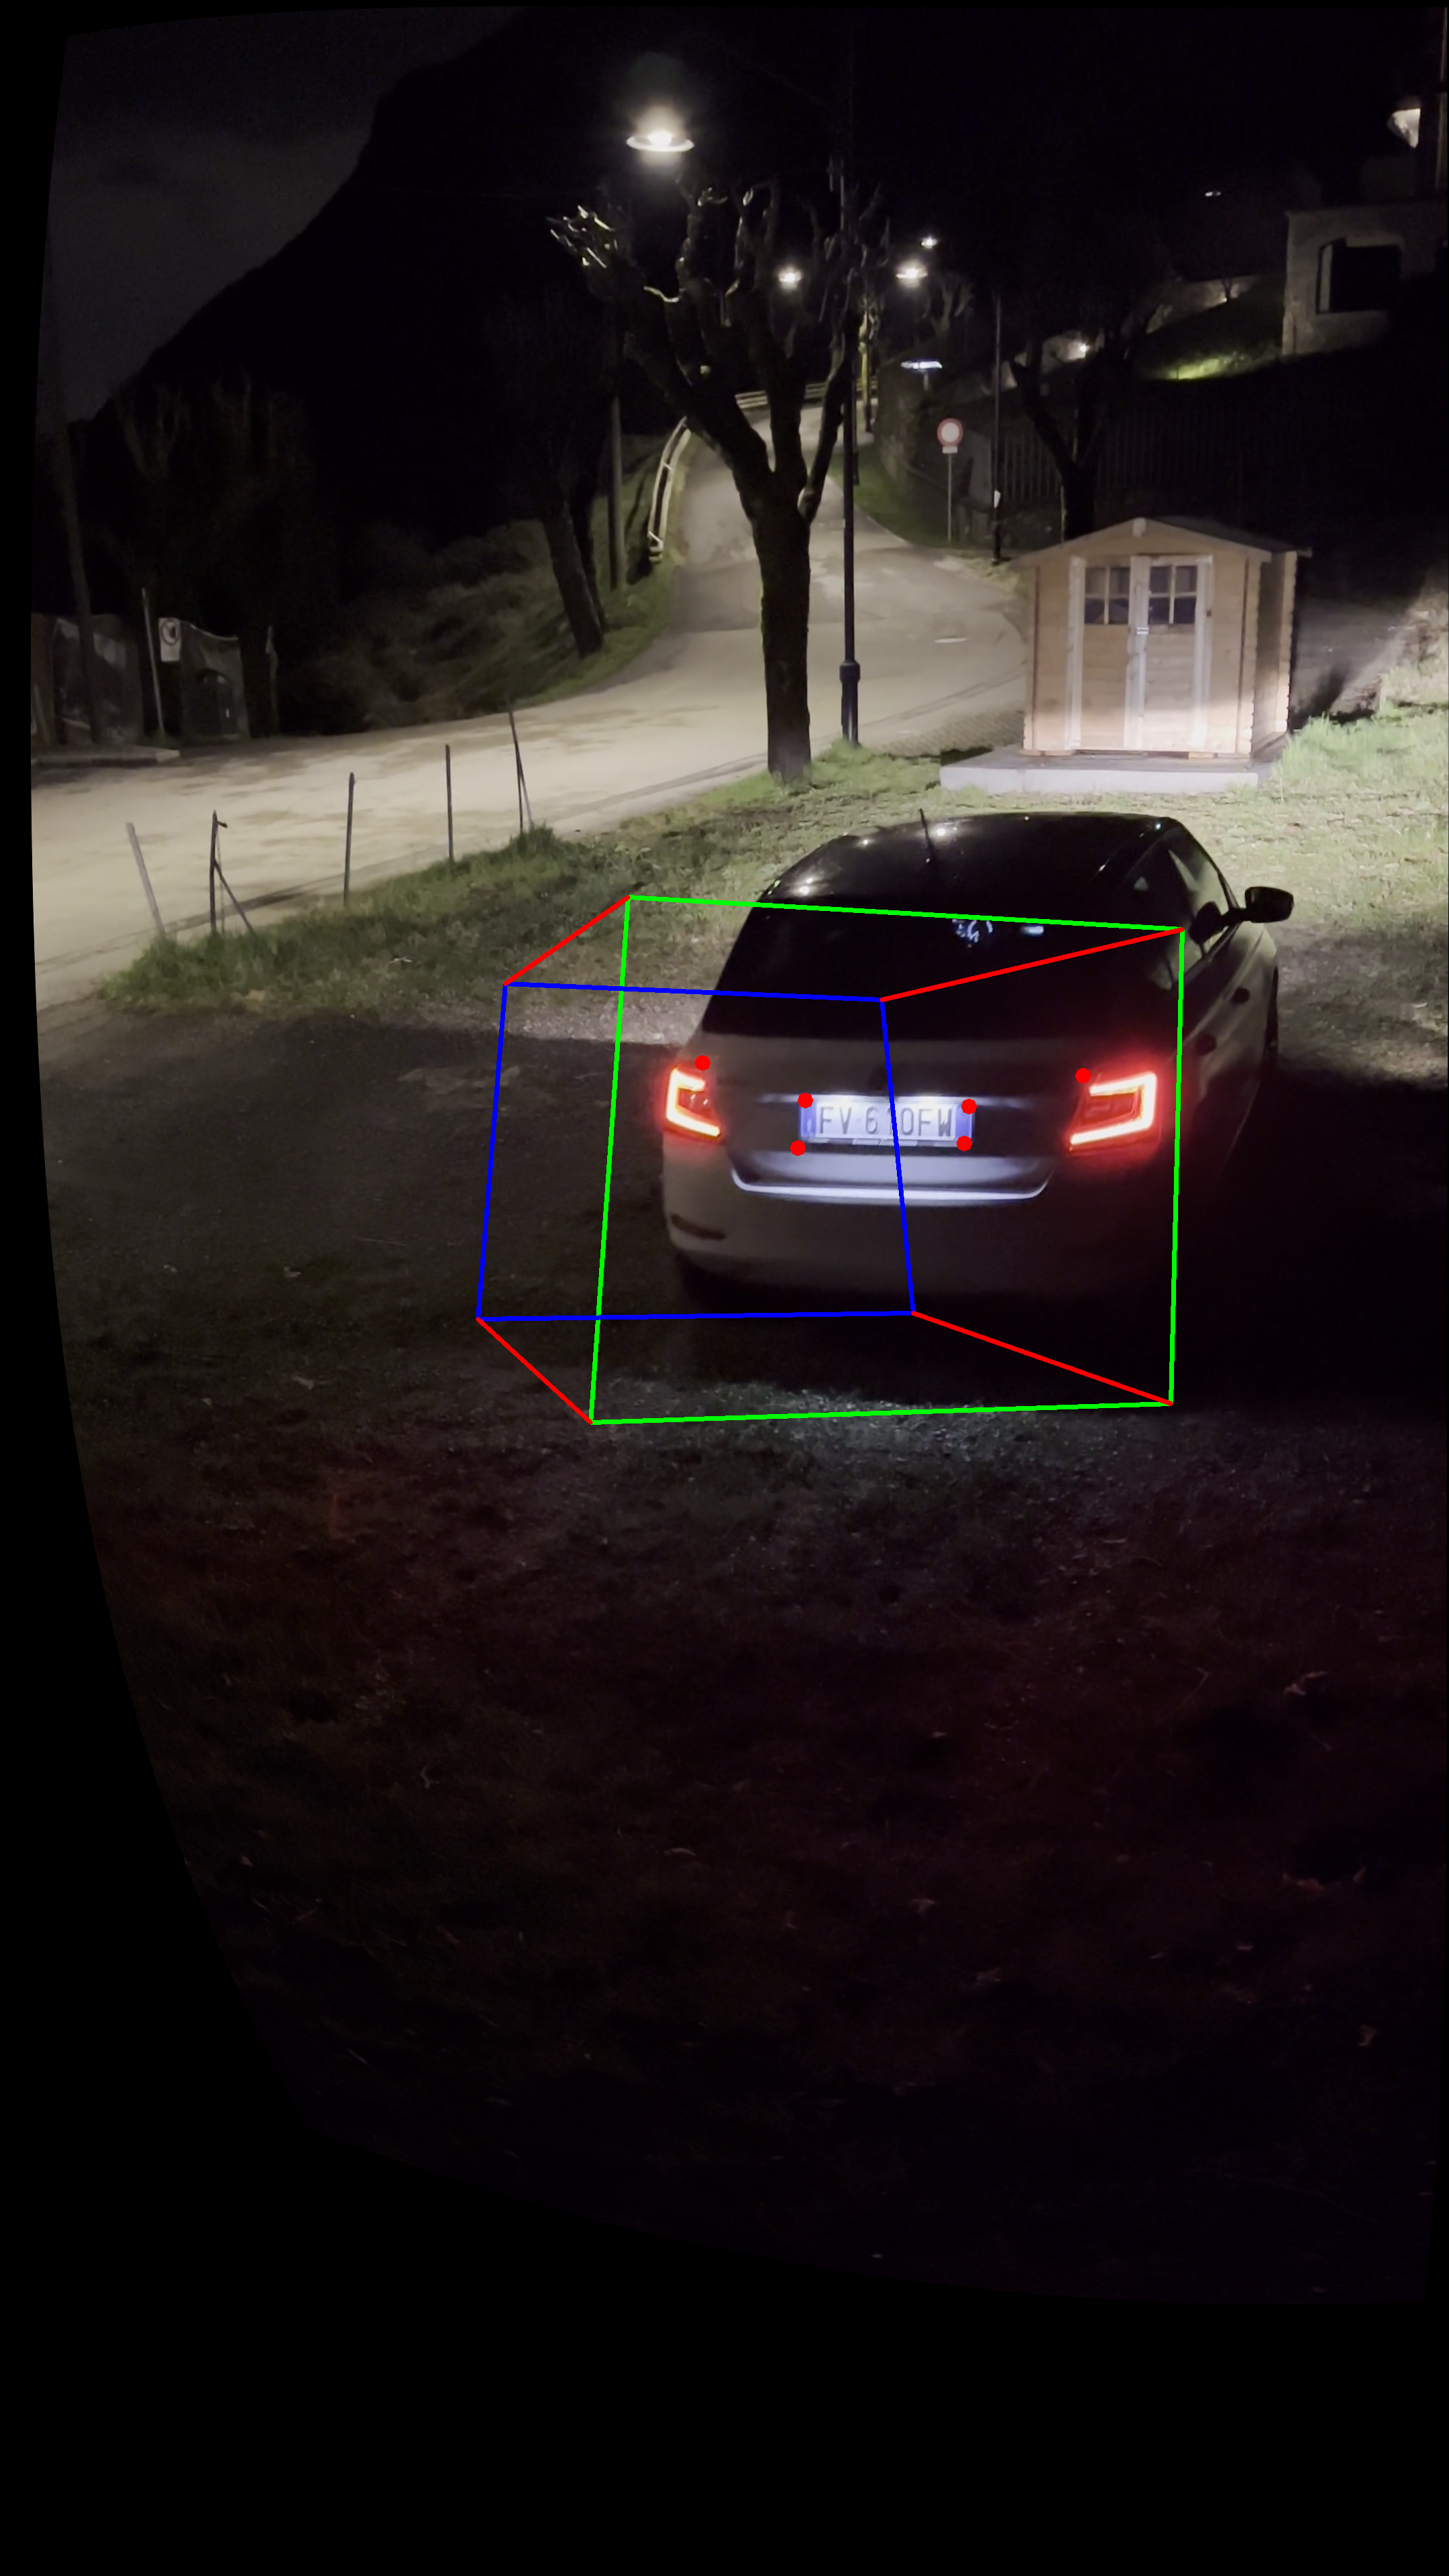
\includegraphics[width=\textwidth]{Images/method4/bbox_4pts_iterative.jpg}
        \caption{4-point PnP using Iterative solver}
    \end{subfigure}
    \hfill
    \begin{subfigure}[b]{0.30\textwidth}
        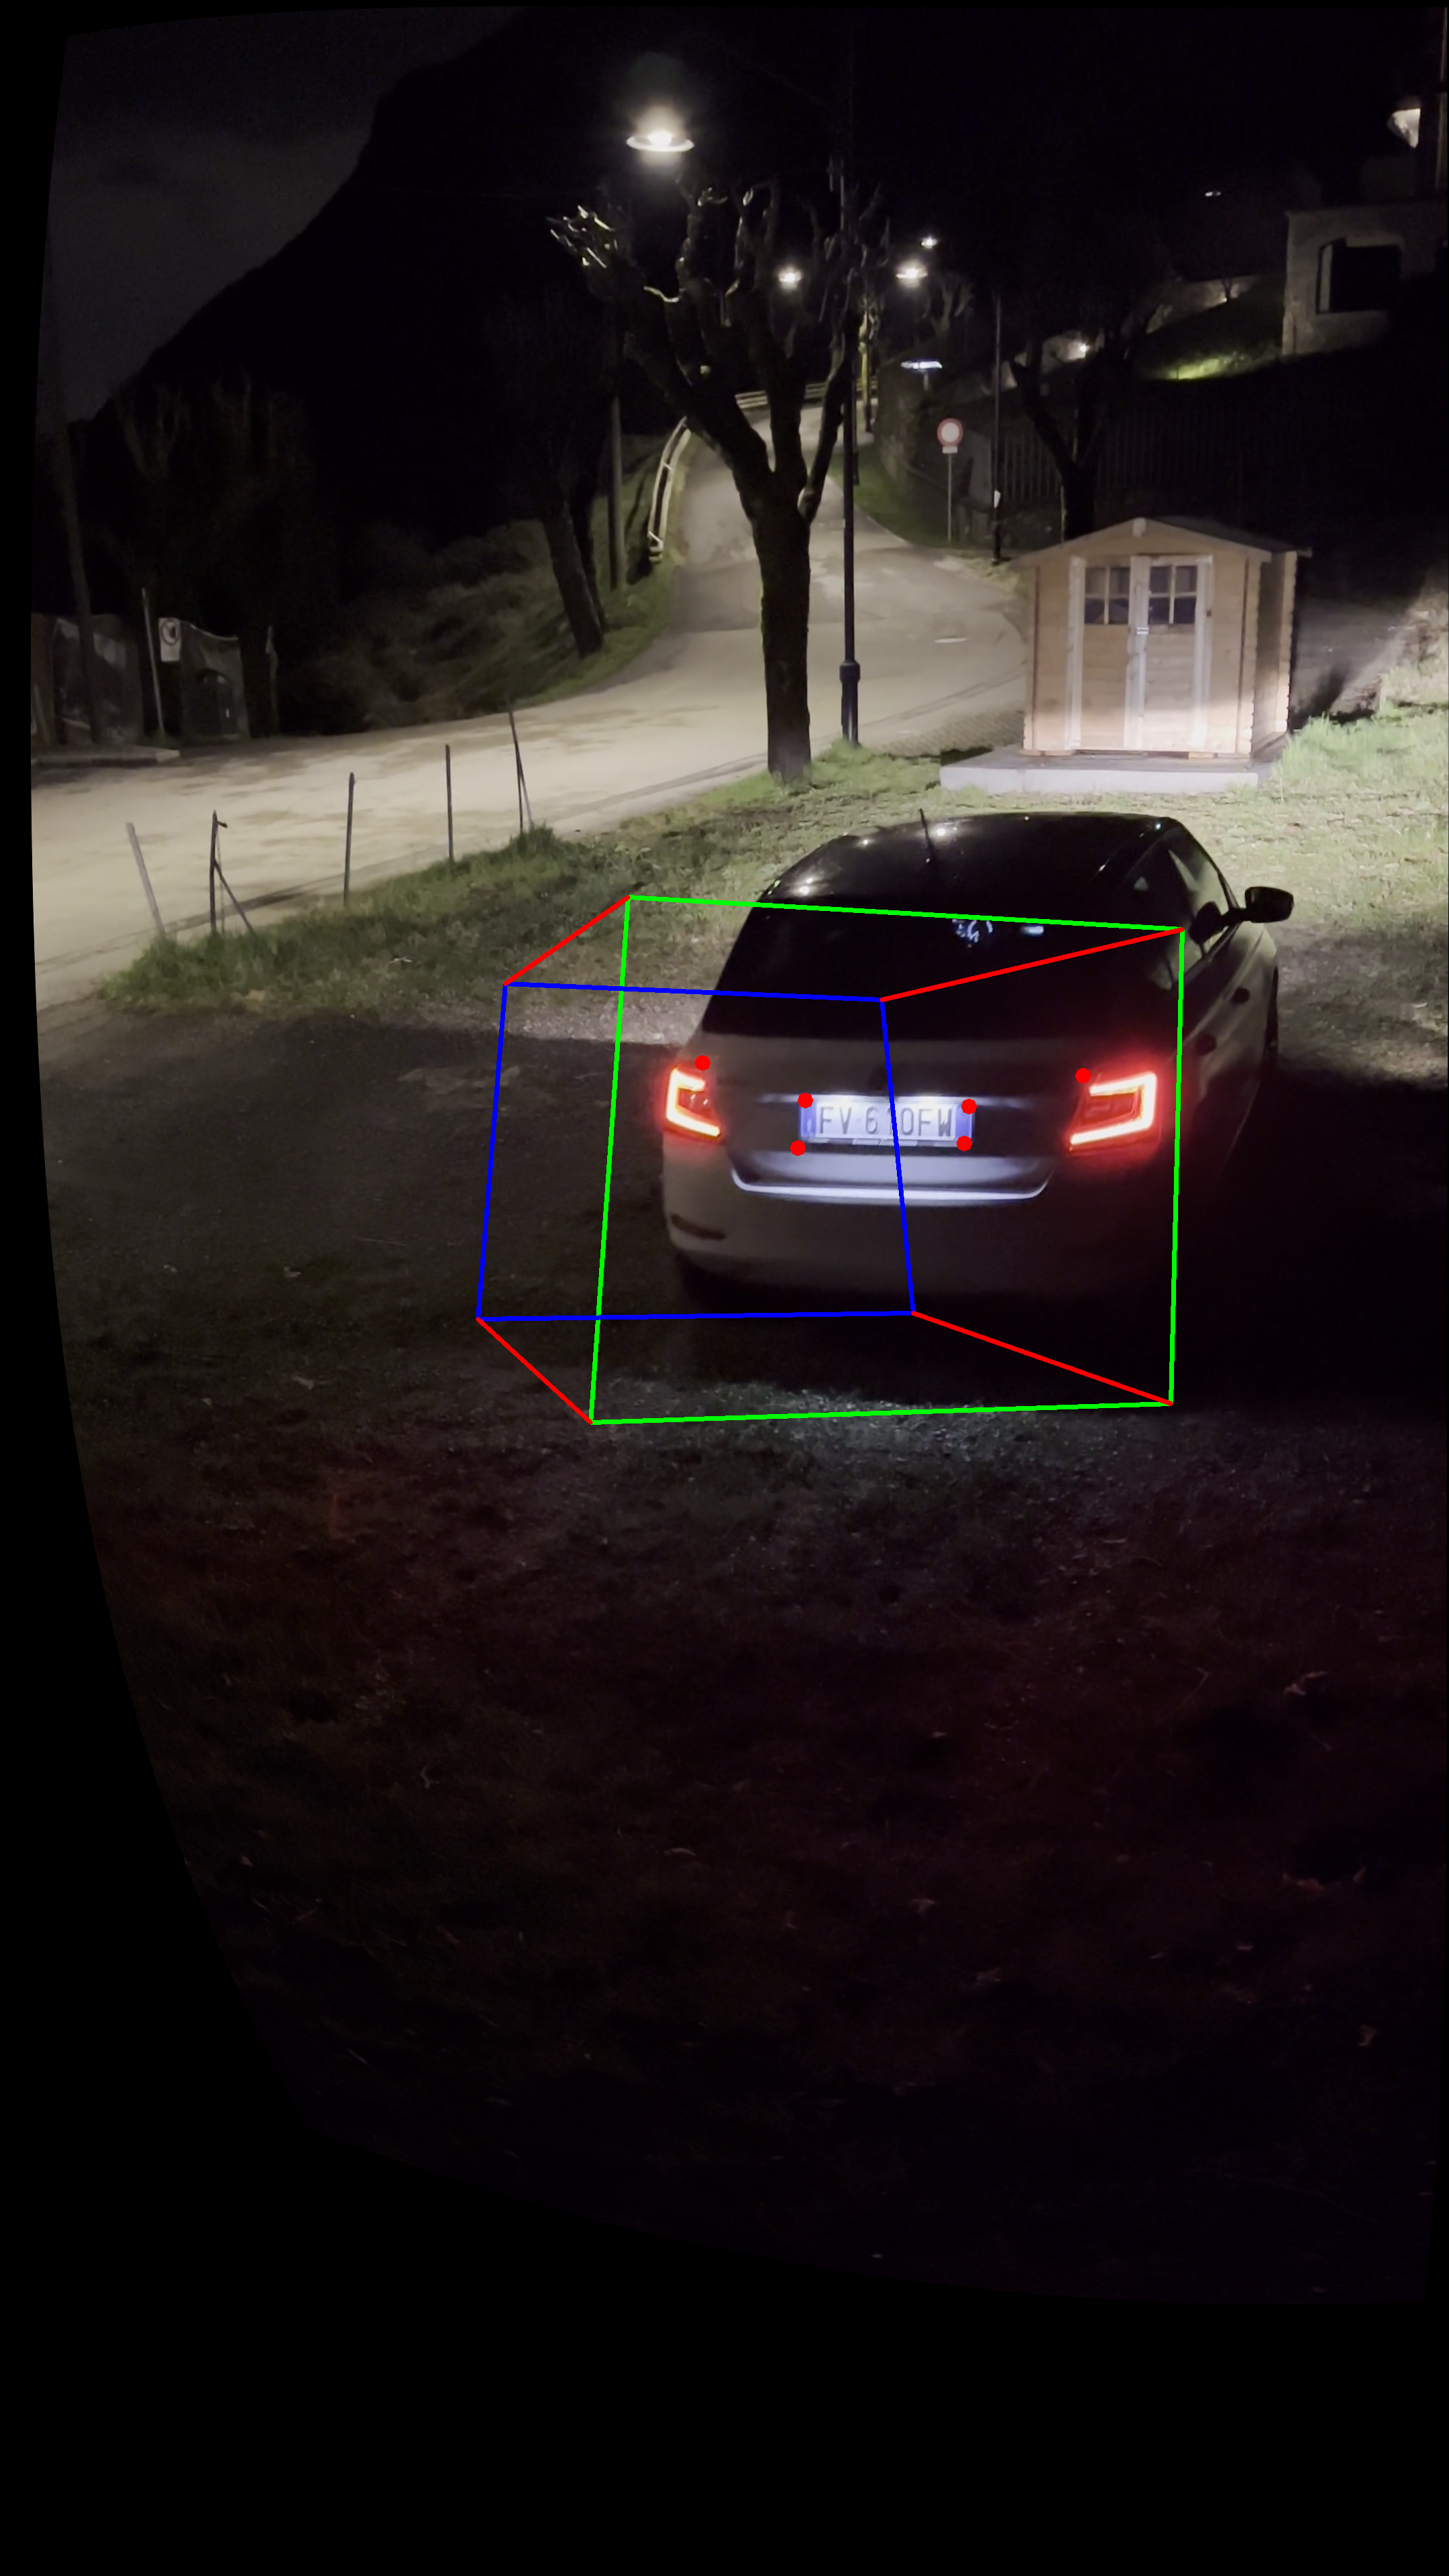
\includegraphics[width=\textwidth]{Images/method4/bbox_4pts_epnp.jpg}
        \caption{4-point PnP using EPnP solver}
    \end{subfigure}
    \hspace*{\fill}
    \caption{Pose estimation comparison using four points and different PnP solvers}
    \label{fig:pnp_4pts}
\end{figure}

Figure~\ref{fig:method4_result} shows the result obtained by extending the model with a fifth point corresponding to the vehicle’s side mirror. The projected bounding box exhibits greater accuracy and spatial consistency, especially in the horizontal extent, validating the benefit of including out-of-plane points in the PnP setup.

\begin{figure}[h]
    \centering
    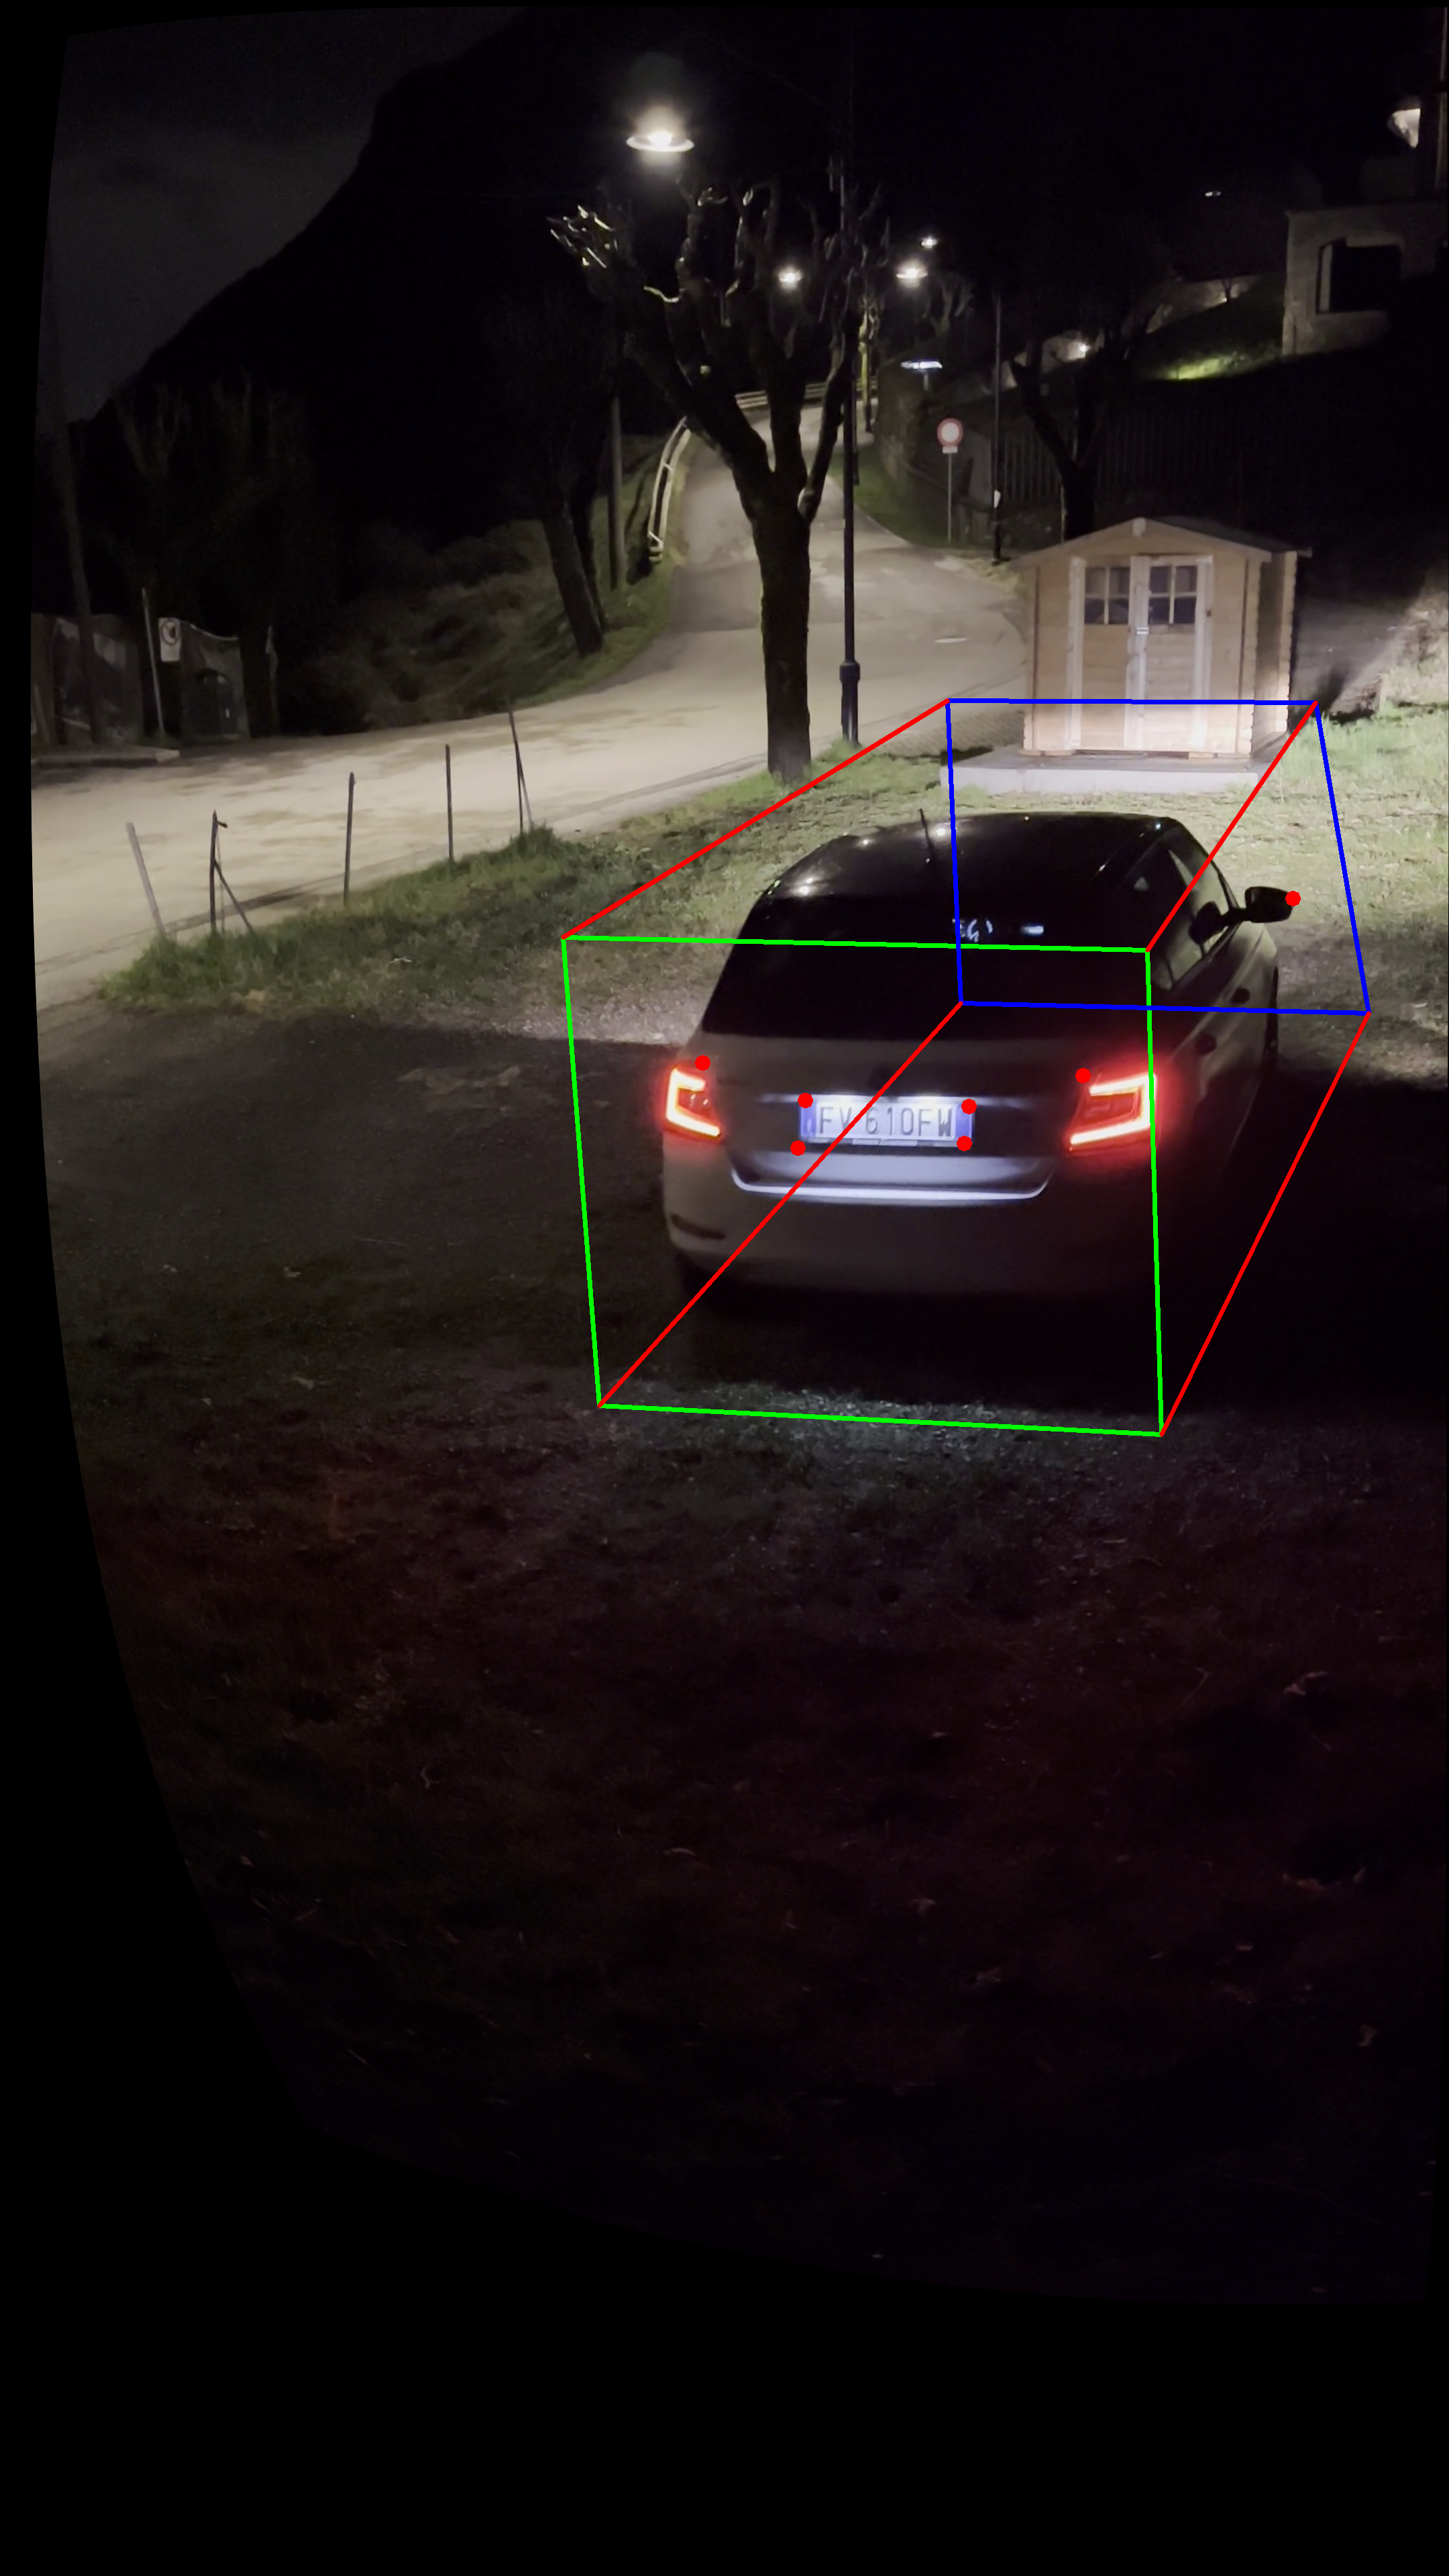
\includegraphics[width=0.35\textwidth]{Images/method4/bbox_5pts_iterative.jpg}
    \caption{Pose estimation using five-point model (license plate, headlights, and mirror)}
    \label{fig:method4_result}
\end{figure}


\chapter{Conclusion}
This chapter summarizes the key findings of the proposed methods for vehicle space occupancy estimation under low-light conditions. It provides a comparative evaluation of the approaches introduced, highlighting their strengths, limitations, and suitability for different scenarios.
\begin{itemize}
    \item \textbf{Method 1} relies on a homography computed from four coplanar vehicle points. While it is simple and computationally efficient, it heavily depends on strong perspective cues. When these cues are weak or absent—such as in frontal or rear views—the method often fails to recover a meaningful pose, limiting its applicability in real-world scenarios.
    \item \textbf{Method 2} builds upon geometric reasoning using vanishing points to estimate the angle between back-projected rays of the two taillights. This method demonstrates high accuracy and reliability when vanishing points can be reliably detected. It avoids strong planar assumptions and performs well under a wide range of perspectives. However, its dependence on precise line detection and vanishing point localization can become a weakness in low-resolution or cluttered images.
    \item \textbf{Method 3} introduces a more sophisticated and iterative approach, reducing the 3D-to-2D problem to a 2D-to-1D projection and refining pose estimates using known vehicle dimensions. It proves to be one of the most robust methods, especially under weak perspective conditions where other methods struggle. Its ability to recover accurate poses from minimal cues makes it highly suitable for real-world deployment. The trade-off lies in the increased computational complexity and reliance on iterative refinement.
    \item \textbf{Method 4} uses the Perspective-n-Point (PnP) framework to estimate vehicle pose from known 3D-to-2D correspondences. While it is highly flexible and accurate when accurate correspondences are available, its performance is sensitive to point detection quality and the assumption of correct vehicle geometry. Additionally, it may not perform well when all visible points lie on the same plane, causing pose ambiguity.
\end{itemize}

In summary, Methods 2 and 3 offer the best balance between accuracy and robustness. Method 2 excels when vanishing points are well-defined, while Method 3 provides resilience in more ambiguous scenes. Methods 1 and 4, although useful in specific contexts, face limitations in generalizability and reliability. Future work may explore hybrid approaches that combine vanishing point geometry with iterative refinement for even greater performance in diverse environments.

\section{Comparison of Results}
The figure \ref{fig:grid_images} shows the comparison between the implemented methods across different frames.

\begin{figure}[htbp]
    \centering
    \setlength{\tabcolsep}{5pt} % column spacing
    \renewcommand{\arraystretch}{1.1} % row height
    \begin{tabular}{c c c c c}
        & \textbf{Frame 4} & \textbf{Frame 8} & \textbf{Frame 12} & \textbf{Frame 16} \\[5pt]

        \raisebox{9\height}{\textbf{Method 1}} &
        \includegraphics[width=0.20\textwidth]{Images/Conclusions/method1/1_frame4.jpg} &
        \includegraphics[width=0.20\textwidth]{Images/Conclusions/method1/1_frame8.jpg} &
        \includegraphics[width=0.20\textwidth]{Images/Conclusions/method1/1_frame12.jpg} &
        \includegraphics[width=0.20\textwidth]{Images/Conclusions/method1/1_frame16.jpg} \\[6pt]

        \raisebox{9\height}{\textbf{Method 2}} &
        \includegraphics[width=0.20\textwidth]{Images/Conclusions/method2/2_frame4.png} &
        \includegraphics[width=0.20\textwidth]{Images/Conclusions/method2/2_frame8.png} &
        \includegraphics[width=0.20\textwidth]{Images/Conclusions/method2/2_frame12.png} &
        \includegraphics[width=0.20\textwidth]{Images/Conclusions/method2/2_frame16.png} \\[6pt]

        \raisebox{9\height}{\textbf{Method 3}} &
        \includegraphics[width=0.20\textwidth]{Images/Conclusions/method3/3_frame4.jpg} &
        \includegraphics[width=0.20\textwidth]{Images/Conclusions/method3/3_frame8.jpg} &
        \includegraphics[width=0.20\textwidth]{Images/Conclusions/method3/3_frame12.jpg} &
        \includegraphics[width=0.20\textwidth]{Images/Conclusions/method3/3_frame16.jpg} \\[6pt]

        \raisebox{9\height}{\textbf{Method 4}} &
        \includegraphics[width=0.20\textwidth]{Images/Conclusions/method4/4_frame4.jpg} &
        \includegraphics[width=0.20\textwidth]{Images/Conclusions/method4/4_frame8.jpg} &
        \includegraphics[width=0.20\textwidth]{Images/Conclusions/method4/4_frame12.jpg} &
        \includegraphics[width=0.20\textwidth]{Images/Conclusions/method4/4_frame16.jpg} \\
    \end{tabular}
    \caption{Comparison of results from different methods across four selected frames}
    \label{fig:grid_images}
\end{figure}


\section{Future Work}

Future work will aim to automate the retrieval of vehicle data by implementing a neural network to recognize license plate characters. The recognized plate will be used to query public databases to obtain the car's make and model. This information will then allow access to 3D CAD model repositories, providing accurate geometrical data without manual input. Additionally, improvements will be made to the robustness of license plate and light detection, using more advanced object detection algorithms to handle challenging conditions such as occlusion or low visibility.



\listoffigures

\bibliography{references}

\end{document}